
\documentclass[12pt,PhD,twoside,openright]{muthesis}

% Packages MU
\usepackage{verbatim}
\usepackage{graphicx}
\usepackage{url} % typeset URL's reasonably
\def\UrlBreaks{\do\/\do-}
\usepackage{listings}

\usepackage{pslatex} % Use Postscript fonts
\usepackage[toc]{}
% Uncomment this to use a glossary
% \usepackage[toc]{glossaries}
% \input{./glossary}
% \makeglossaries

%%%%%%%%%%%%%%%%%%%%%%
\usepackage{graphicx,latexsym}
\usepackage{amsmath}
\usepackage{amssymb,amsthm}
\usepackage{longtable,booktabs,setspace}
% \usepackage{chemarr} %% Useful for one reaction arrow, useless if you're not a chem major
% \usepackage[hyphens]{url}
% Added by CII
\usepackage[anythingbreaks]{}
\usepackage{hyperref}
\hypersetup{colorlinks = false}
\renewcommand{\UrlBreaks}{\do\/\do\a\do\b\do\c\do\d\do\e\do\f\do\g\do\h\do\i\do\j\do\k\do\l\do\m\do\n\do\o\do\p\do\q\do\r\do\s\do\t\do\u\do\v\do\w\do\x\do\y\do\z\do\A\do\B\do\C\do\D\do\E\do\F\do\G\do\H\do\I\do\J\do\K\do\L\do\M\do\N\do\O\do\P\do\Q\do\R\do\S\do\T\do\U\do\V\do\W\do\X\do\Y\do\Z\do\0\do\1\do\2\do\3\do\4\do\5\do\6\do\7\do\8\do\9\do\%\do\.\do\-}

\renewcommand{\chapterautorefname}{Chapter}

\usepackage{lmodern}
\usepackage{float}
\floatplacement{figure}{H}
% End of CII addition
\usepackage{rotating}


\usepackage{natbib}
%%% --- The following two lines are what needs to be added --- %%%
%\setcounter{biburllcpenalty}{7000}
%\setcounter{biburlucpenalty}{8000}
% Comment out the natbib line above and uncomment the following two lines to use the new
% biblatex-chicago style, for Chicago A. Also make some changes at the end where the
% bibliography is included.
%\usepackage{biblatex-chicago}
%\bibliography{thesis}


% Added by CII (Thanks, Hadley!)
% Use ref for internal links
% \renewcommand{\hyperref}[2][???]{\autoref{#1}}
% \def\chapterautorefname{Chapter}
% \def\sectionautorefname{Section}
% \def\subsectionautorefname{Subsection}
% End of CII addition

% Added by CII
\usepackage{caption}
% \captionsetup{width=5in}
% End of CII addition

% \usepackage{times} % other fonts are available like times, bookman, charter, palatino

% Syntax highlighting #22
  \usepackage{color}
  \usepackage{fancyvrb}
  \newcommand{\VerbBar}{|}
  \newcommand{\VERB}{\Verb[commandchars=\\\{\}]}
  \DefineVerbatimEnvironment{Highlighting}{Verbatim}{commandchars=\\\{\}}
  % Add ',fontsize=\small' for more characters per line
  \usepackage{framed}
  \definecolor{shadecolor}{RGB}{248,248,248}
  \newenvironment{Shaded}{\begin{snugshade}}{\end{snugshade}}
  \newcommand{\AlertTok}[1]{\textcolor[rgb]{0.94,0.16,0.16}{#1}}
  \newcommand{\AnnotationTok}[1]{\textcolor[rgb]{0.56,0.35,0.01}{\textbf{\textit{#1}}}}
  \newcommand{\AttributeTok}[1]{\textcolor[rgb]{0.77,0.63,0.00}{#1}}
  \newcommand{\BaseNTok}[1]{\textcolor[rgb]{0.00,0.00,0.81}{#1}}
  \newcommand{\BuiltInTok}[1]{#1}
  \newcommand{\CharTok}[1]{\textcolor[rgb]{0.31,0.60,0.02}{#1}}
  \newcommand{\CommentTok}[1]{\textcolor[rgb]{0.56,0.35,0.01}{\textit{#1}}}
  \newcommand{\CommentVarTok}[1]{\textcolor[rgb]{0.56,0.35,0.01}{\textbf{\textit{#1}}}}
  \newcommand{\ConstantTok}[1]{\textcolor[rgb]{0.00,0.00,0.00}{#1}}
  \newcommand{\ControlFlowTok}[1]{\textcolor[rgb]{0.13,0.29,0.53}{\textbf{#1}}}
  \newcommand{\DataTypeTok}[1]{\textcolor[rgb]{0.13,0.29,0.53}{#1}}
  \newcommand{\DecValTok}[1]{\textcolor[rgb]{0.00,0.00,0.81}{#1}}
  \newcommand{\DocumentationTok}[1]{\textcolor[rgb]{0.56,0.35,0.01}{\textbf{\textit{#1}}}}
  \newcommand{\ErrorTok}[1]{\textcolor[rgb]{0.64,0.00,0.00}{\textbf{#1}}}
  \newcommand{\ExtensionTok}[1]{#1}
  \newcommand{\FloatTok}[1]{\textcolor[rgb]{0.00,0.00,0.81}{#1}}
  \newcommand{\FunctionTok}[1]{\textcolor[rgb]{0.00,0.00,0.00}{#1}}
  \newcommand{\ImportTok}[1]{#1}
  \newcommand{\InformationTok}[1]{\textcolor[rgb]{0.56,0.35,0.01}{\textbf{\textit{#1}}}}
  \newcommand{\KeywordTok}[1]{\textcolor[rgb]{0.13,0.29,0.53}{\textbf{#1}}}
  \newcommand{\NormalTok}[1]{#1}
  \newcommand{\OperatorTok}[1]{\textcolor[rgb]{0.81,0.36,0.00}{\textbf{#1}}}
  \newcommand{\OtherTok}[1]{\textcolor[rgb]{0.56,0.35,0.01}{#1}}
  \newcommand{\PreprocessorTok}[1]{\textcolor[rgb]{0.56,0.35,0.01}{\textit{#1}}}
  \newcommand{\RegionMarkerTok}[1]{#1}
  \newcommand{\SpecialCharTok}[1]{\textcolor[rgb]{0.00,0.00,0.00}{#1}}
  \newcommand{\SpecialStringTok}[1]{\textcolor[rgb]{0.31,0.60,0.02}{#1}}
  \newcommand{\StringTok}[1]{\textcolor[rgb]{0.31,0.60,0.02}{#1}}
  \newcommand{\VariableTok}[1]{\textcolor[rgb]{0.00,0.00,0.00}{#1}}
  \newcommand{\VerbatimStringTok}[1]{\textcolor[rgb]{0.31,0.60,0.02}{#1}}
  \newcommand{\WarningTok}[1]{\textcolor[rgb]{0.56,0.35,0.01}{\textbf{\textit{#1}}}}




% if you're writing a thesis in an interdisciplinary major,
% uncomment the line below and change the text as appropriate.
% check the Senior Handbook if unsure.
%\thedivisionof{The Established Interdisciplinary Committee for}
% if you want the approval page to say "Approved for the Committee",
% uncomment the next line
%\approvedforthe{Committee}

% Added by CII
%%% Copied from knitr
%% maxwidth is the original width if it's less than linewidth
%% otherwise use linewidth (to make sure the graphics do not exceed the margin)
% \makeatletter
% \def\maxwidth{ %
%   \ifdim\Gin@nat@width>\linewidth
%     \linewidth
%   \else
%     \Gin@nat@width
%   \fi
% }
% \makeatother

% \renewcommand{\contentsname}{Table of Contents}
% End of CII addition

% \setlength{\parskip}{0pt}

% Added by CII
% 
\providecommand{\tightlist}{%
  \setlength{\itemsep}{0pt}\setlength{\parskip}{0pt}}

	\newcommand{\txt}[1]{\textrm{#1}}

 \def\logit{\txt{logit}}

 \newcommand{\sfrac}[2]{\;^{#1}/_{#2}}
	\usepackage{amsmath}
 \usepackage{rotating}
 \usepackage{booktabs}
 \usepackage{longtable}
 \usepackage{array}
 \usepackage{multirow}
 \usepackage{wrapfig}
 \usepackage{float}
 \usepackage{colortbl}
 \usepackage{pdflscape}
 \usepackage{tabu}
 \usepackage{threeparttable}
 \usepackage{threeparttablex}
 \usepackage[normalem]{ulem}
 \usepackage{makecell}
 \usepackage{xcolor}

\newlength{\cslhangindent}
\setlength{\cslhangindent}{1.5em}
\newenvironment{cslreferences}%
  {}%
  {\par}
  

\begin{document}

\title{Multi-State Clinical Prediction Models in Renal Replacement Therapy}
\author{Michael Andrew Barrowman}
\principaladviser{}
\faculty{}
\school{}
\beforeabstract

\prefacesection{Abstract}
The preface pretty much says it all.

\par

Second paragraph of abstract starts here. Prelim

\afterabstract

\prefacesection{Acknowledgements}

\begingroup

\setlength{\parskip}{15pt}
\setlength{\parindent}{0pt}
I would like to thank my wife, Rachel, for her constant support throughout my studies. She acted as sounding board for my most boring of thoughts and allowed me to rant and rave about statistical models in every way possible. She endured my frustrations when something wasn't working and encouraged me when my optimism turned to pesimism.

\par

My thanks also go to my children, Matilda and Theodore, who were an everlasting source of happiness and reprieve from my work. Acting as a distraction (in the best and worst ways) and an incentive.

\par

My everlasting gratitude will always lie with my parents, Brenda and Andy, who have allowed me to be myself and to find my own path. They never pushed me into something that I didn't want to do, but also guided me towards what I would be good at.

\par

My final thanks go to my PhD supervisors, Matt, Niels, Glen and Mark, who have provided advice and feedback for over four years.
\endgroup
\afterpreface

\hypertarget{chap-dev-paper}{%
\chapter{Development and External Validation of a Multi-State Clinical Prediction Model for Chronic Kidney Disease Patients Progressing onto Renal Replacement Therapy and Death}\label{chap-dev-paper}}

\hypertarget{introduction}{%
\section{Introduction}\label{introduction}}

A clinical prediction model (CPM) is a tool which provides patients and clinicians with a measure of how likely a patient is to suffer a specific clinical condition, more specifically, a prognostic model allows the prediction of future events {[}\protect\hyperlink{ref-steyerberg_prognosis_2013}{1}{]}. CPMs use data from previous patients to estimate the outcomes of an individual patient. Prognostic models are used in clinical practice to influence treatment decisions such as the prescribing of statins for cardiovascular disease via the application of the QRISK models {[}\protect\hyperlink{ref-hippisley-cox_development_2017}{2}{]}.

Within Chronic Kidney Disease (CKD), prognostic models have been developed to predict mortality {[}\protect\hyperlink{ref-johnson_predicting_2007}{3}{]}--{[}\protect\hyperlink{ref-wick_clinical_2017}{7}{]}, ESRD {[}\protect\hyperlink{ref-landray_prediction_2010}{4}{]}, the commencements of RRT {[}\protect\hyperlink{ref-marks_looking_2015}{6}{]}, {[}\protect\hyperlink{ref-johnson_predicting_2008}{8}{]}--{[}\protect\hyperlink{ref-kulkarni_transition_2017}{10}{]} or mortality after beginning dialysis {[}\protect\hyperlink{ref-floege_development_2015}{11}{]}--{[}\protect\hyperlink{ref-cao_predicting_2015}{13}{]}. Some previous models have used the commencement of RRT as a proxy for ESRD {[}\protect\hyperlink{ref-tangri_predictive_2011}{14}{]}--{[}\protect\hyperlink{ref-tangri_dynamic_2017}{16}{]}, while others have investigated the occurrence of cardiovascular events within CKD patients{[}\protect\hyperlink{ref-shlipak_cardiovascular_2005}{17}{]}--{[}\protect\hyperlink{ref-mcmurray_predictors_2011}{19}{]}. Reviews by Grams \& Coresh {[}\protect\hyperlink{ref-grams_assessing_2013}{20}{]}, Tangri et al {[}\protect\hyperlink{ref-tangri_risk_2013}{21}{]} and Ramspek et al {[}\protect\hyperlink{ref-ramspek_prediction_2017}{22}{]}, which explored the different aspects of assessing risk amongst CKD or RRT patients, found that the current landscape of CKD prediction models is lacking from both a methodological and clinical perspective {[}\protect\hyperlink{ref-collins_transparent_2015}{23}{]}, {[}\protect\hyperlink{ref-bouwmeester_reporting_2012-1}{24}{]}.

Methodologically, the majority of existing CKD prediction models fail to account for completing events {[}\protect\hyperlink{ref-bansal_development_2015}{5}{]}, {[}\protect\hyperlink{ref-wick_clinical_2017}{7}{]}, {[}\protect\hyperlink{ref-perotte_risk_2015}{25}{]}, have high risks of bias {[}\protect\hyperlink{ref-johnson_predicting_2007}{3}{]}, {[}\protect\hyperlink{ref-landray_prediction_2010}{4}{]}, {[}\protect\hyperlink{ref-johnson_predicting_2008}{8}{]} or are otherwise flawed compared to modern clinical prediction standards {[}\protect\hyperlink{ref-steyerberg_prognosis_2013}{1}{]}, {[}\protect\hyperlink{ref-collins_transparent_2015}{23}{]}

In 2013, Begun et al {[}\protect\hyperlink{ref-begun_identification_2013}{26}{]} developed a multi-State model for assessing population-level progression through the severity stages of CKD (III-V), RRT and/or death, which can be used to provide a broad statement regarding a patient's future. In 2014, Allen et al {[}\protect\hyperlink{ref-allen_chronic_2014}{27}{]} applied a similar model to liver transplant recipients and their progression through the stages of CKD with a focus on the predictions of measured vs estimated glomerular filtration rate (mGFR vs eGFR). In 2017, Kulkarni et al {[}\protect\hyperlink{ref-kulkarni_transition_2017}{10}{]} developed an MSM focusing on the categories of Calculated Panel Reactive Antibodies (CPRA) and kidney transplant and/or death.

Most recently, in 2018, Grams et al {[}\protect\hyperlink{ref-grams_predicting_2018}{28}{]} developed a multinomial clinical prediction model for CKD patients which focused on the occurrence of RRT and/or cardiovascular events. As of the publication of this paper, this is the only currently existing CPMs of this kind for CKD patients.

However, the first three of these existing models (Begun, Allen and Kulkarni) categorise continuous variables to define their states at specific cut-offs and this has been shown to be inefficient when modelling {[}\protect\hyperlink{ref-altman_problems_1994-1}{29}{]}--{[}\protect\hyperlink{ref-weinberg_how_1995}{47}{]}. These kinds of cut-offs can be useful when informing patients and clinicians of a patient's diagnosis and to coincide with policy, but inherently cause a loss of information when done before the data analysis stage and so these models go against current statistical recommendations {[}\protect\hyperlink{ref-altman_problems_1994-1}{29}{]}--{[}\protect\hyperlink{ref-weinberg_how_1995}{47}{]}. These kinds of assumptions are also subject to measurement error {[}\protect\hyperlink{ref-van_smeden_reflection_2019}{48}{]} and interval censoring {[}\protect\hyperlink{ref-sun_interval_2005}{49}{]}, i.e.~we do not know when exactly when a patient moved from CKD Stage III to CKD Stage IV, or whether drop in estimated Glomerular Function Rate (eGFR) was temporary or inaccurate. For example, Kulkarni {[}\protect\hyperlink{ref-kulkarni_transition_2017}{10}{]} assumes that a patient with an CPRA of (5\%) is the same as a patient with an CPRA of (75\%) and that a patient with an CPRA of (89.9\%) is vastly different from a patient with an CPRA of (90\%). Moreover, none of these models have undergone any validation process, whether internal or external {[}\protect\hyperlink{ref-altman_prognosis_2009}{50}{]}.

It is also important to note that although these models can be used to predict patient outcomes, they were not designed to produce individualised patient predictions as is a key aspect of a clinical prediction model; they were designed to assess the methodological advantages of MSMs in this medical field, to describe the prevalence of over time of different CKD stages and to produce population level predictions for patients with different levels of panel-reactive antibodies {[}\protect\hyperlink{ref-royston_prognosis_2009}{51}{]}.

The fourth model (Grams), is presented as a Multi-State Model and the transitions involved were studied and defined, however the underlying statistical model is a pair of multinomial logistic models analysed at 2 and 4 years. The major downside of this model is that it can only produce predictions at those predefined time points and it assumes homogeneity of transition times. For example, the first model assumes that a patient who began RRT 1 month after study entry is the same as one who began after 1 year \& 11 months into the study and then the second model assumes these patients are the same as one who begins RRT at 3 years and 11 months.

Therefore, the aim of this study was to improve on previous efforts to model a patient's pathways through a Multi-State Model by choosing transition points which can be exactly identified and include states which produce a drastic difference in patient characteristics. Our modeling techniques allow for individual predictions (using a proportional hazards model) of multiple outcomes (using MSMs) at any time point (using cubic splines). The models produced by this process will then be validated, both internally and externally, to compare their results and demonstrate the transportability of the (statistically robust) clinical prediction models. We report our work in line with the TRIPOD guidelines for development and validation of clinical prediction models {[}\protect\hyperlink{ref-collins_transparent_2015}{23}{]}, {[}\protect\hyperlink{ref-moons_transparent_2015}{52}{]}.

\hypertarget{methods}{%
\section{Methods}\label{methods}}

\hypertarget{data-sources}{%
\subsection{Data Sources}\label{data-sources}}

The models were developed using data from the Salford Kidney Study (SKS) cohort of patients (previously named the CRISIS cohort), established in the Department of Renal Medicine, Salford Royal NHS Foundation Trust (SRFT). The SKS is a large longitudinal CKD cohort recruiting CKD patients since 2002. This cohort collects detailed annualised phenotypic and laboratory data, and plasma, serum and whole blood stored at -80\textdegree C for biomarker and genotypic analyses. Recruitment of patients into SKS has been described in multiple previous studies {[}\protect\hyperlink{ref-hoefield_factors_2010}{53}{]}, {[}\protect\hyperlink{ref-chinnadurai_increased_2019-1}{54}{]} and these have included a CKD progression prognostic factor study and to evidence the increased risk of cardiovascular events in diabetic kidney patients. In brief, any patient referred to Salford renal service (catchment population 1.5 million) who is 18 years or over and has an eGFR measurement of less than \(60\textrm{ml}/\textrm{min}/1.73\textrm{m}^2\) (calculated using the CKD-EPI formula {[}\protect\hyperlink{ref-levey_new_2009}{55}{]}) was approached to be consented for the study participation.

At baseline, the data, including demographics, comorbidities, physical parameters, lab results and primary renal diagnosis are recorded in the database. Patients undergo an annual study visit and any changes to these parameters are captured. All data except blood results are collected via questionnaire by a dedicated team of research nurses. Blood results (baseline and annualised), first RRT modality and mortality outcome data are directly transferred to the database from Salford's Integrated Record (SIR) {[}\protect\hyperlink{ref-new_obtaining_2014}{56}{]}. eGFR, uPCR, comorbidity and blood results were measured longitudinally throughout a patient's time within the cohort.

Due to limitations in our data, we were agnostic to how long since patients were diagnosed with CKD. Therefore, we defined a patient's start date for our model as their first date after consent at which their eGFR was recorded to be below \(60\textrm{ml}/\textrm{min}/1.73\textrm{m}^2\). Some patients consented with an eGFR that was already below 60, and some entered our study later when their eGFR was measured to be below 60. This implies that our models includes both patient who have recently been diagnosed with CKD (\(\textrm{eGFR} \lessapprox 60\)) \emph{and} those that have been suffering with CKD for an arbitrary amount of time. This timelessness of the model means it can be applied to any patient at any time during their CKD journey.

This allows for a wider range of baseline eGFR measurements and patients who have been suffering from CKD, translating to a model which can be applied to

All patients registered in the database between October 2002 and December 2016 with available data were included in this study. As this is a retrospective convenience sample, no sample size calculations were performed prior to recruitment. All patients were followed-up within SKS until the end-points of RRT, death or loss to follow-up or were censored at their last interaction with the healthcare system prior to December 2017. Date of death for patients who commenced RRT was also available within SIR and so also included in the SKS database.

For external validation of the model, we extracted an independent cohort from the West of Scotland Electronic Renal Patient Record (SERPR). Our extract of SERPR contains all patients known to the Glasgow and Forth Valley renal service who had an eGFR measure of less than \(60\textrm{ml}/\textrm{min}/1.73m^2\) between January 2006 and January 2016. This cohort has been previously used in Chronic Kidney Disease Prognosis consortium studies investigating outcomes in patients with CKD {[}\protect\hyperlink{ref-matsushita_cohort_2013}{57}{]} and a similar cohort has been used for the analysis of skin tumours amongst renal transplant patients. Use of anonymised data from this database has been approved by the West of Scotland Ethics Committee for use of NHS Greater Glasgow and Clyde `Safe Haven' data for research.

Both the internal and external validation cohort were used as part of the multinational validation cohort used by Grams et al in their multinomial CPM discussed above {[}\protect\hyperlink{ref-grams_predicting_2018}{28}{]}. In SERPR, start dates were calculated to be the first time point where the following conditions were met:
\begin{itemize}
\tightlist
\item
  eGFR is measured at less than 60
\item
  There is at least one prior eGFR measurement
\item
  Patient is 18 or over
\item
  Patient is not enduring an AKI {[}\protect\hyperlink{ref-forni_renal_2017-1}{58}{]}, {[}\protect\hyperlink{ref-noauthor_kdigo_2012}{59}{]}.
\end{itemize}
The second requirement was implemented to avoid a bias in the eGFR Rate. eGFR Rate is a measure of the change in eGFR over time and is calculated as the difference between the most recent two eGFR measurements divided by the time between them. For patients who entered the system with an \(\textrm{eGFR} < 60\), their eGFR Rate would be unavailable (i.e.~missing). Otherwise, patient eGFRs would \emph{have} to drop to below 60 and thus eGFR Rate would be negative. {[}\textbf{I feel like this bias should have a name, but can't think what to search to find it}{]}

\hypertarget{model-design}{%
\subsection{Model Design}\label{model-design}}

Three separate models were developed, so we could determine a clinically viable model while maintaining model parsimony as much as possible: a Two-State, Three-State and Five-State model, each building on the previous models' complexity (see figure \ref{fig:State-Diagram}). The Two-State model was a traditional survival analysis where a single event (death) is considered. The Three-State model expanded on this, by splitting the Alive state into transient states of (untreated) CKD and (first) RRT; patients can therefore transition from CKD to Death or CKD to RRT, and then onto RRT to Death. The Five-State model stratifies the RRT state into HD, PD and Tx and allows similar transitions into and out of the RRT states; however, the transition from Tx to Death was not considered as it was anticipated a priori that there would be insufficient patients undergoing this transition and that the process of undergoing a transplant would be medically transformative and so it would be inappropriate to assume shared parameters before and after the transition (i.e.~Tx was modelled as a second absorbing state).
\begin{figure}

{\centering 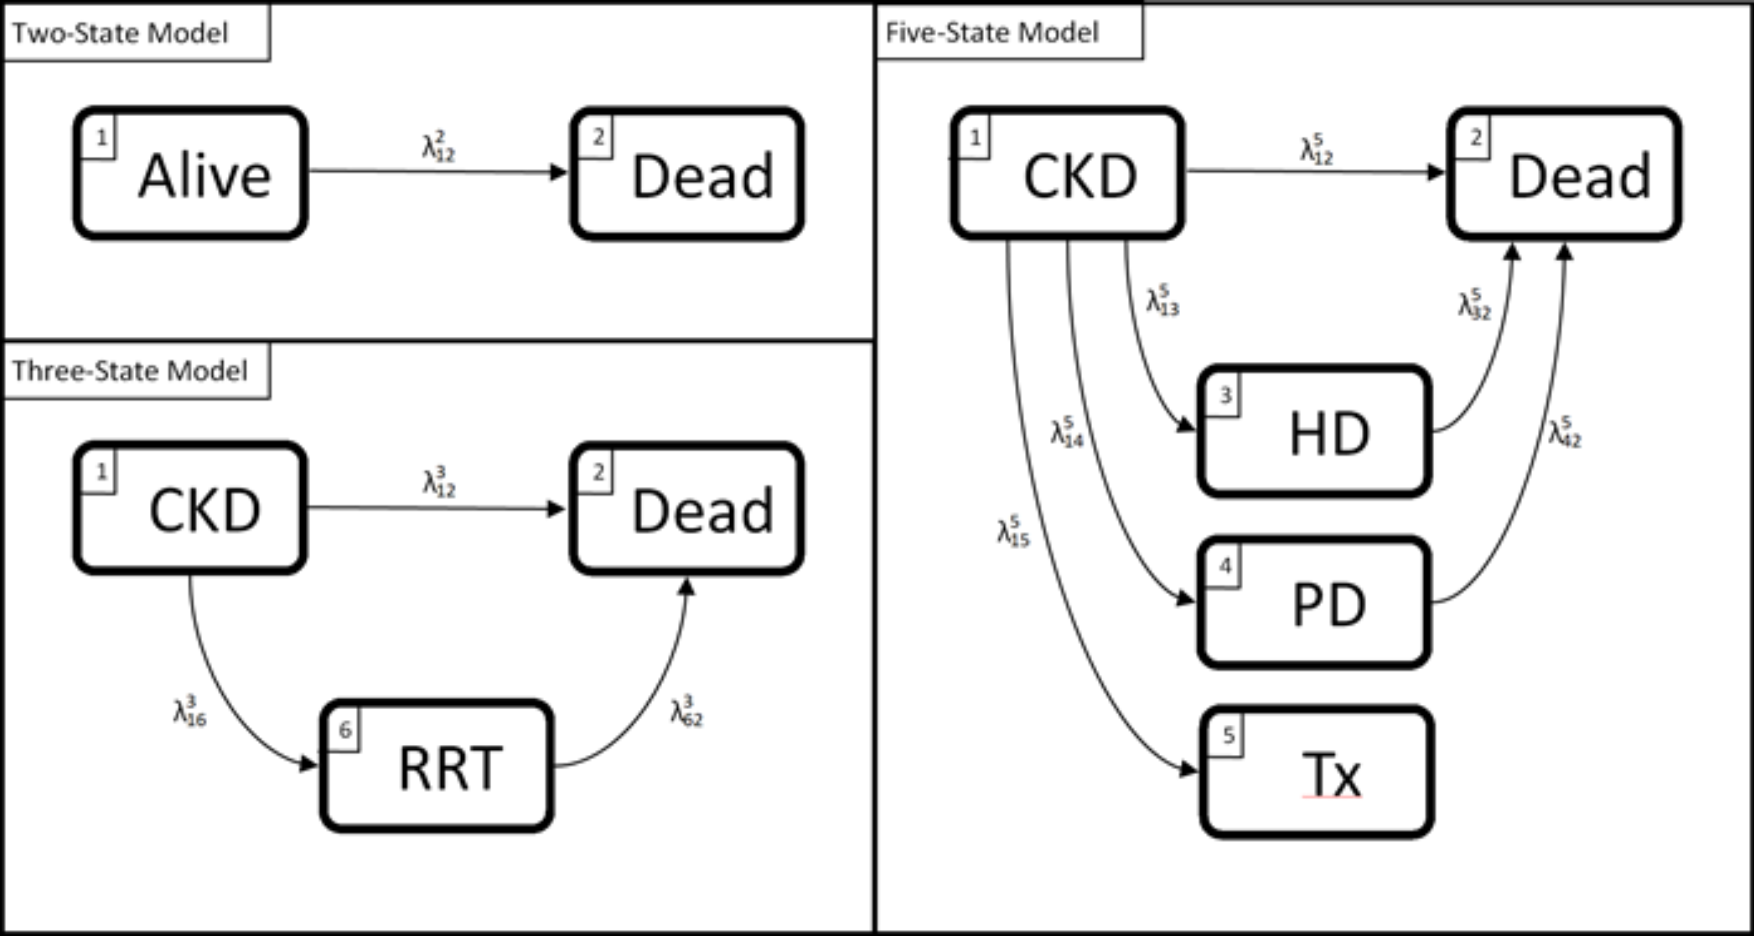
\includegraphics[width=0.9\linewidth]{figure/Dev_Paper_State_Diagrams} 

}

\caption{Diagram of the three models, the states being modelled and relevant transitions}\label{fig:State-Diagram}
\end{figure}
The models were developed and validated as discussed in the Supplementary materials appendix \{\#chap-dev-paper-supp\}.

\hypertarget{example}{%
\subsection{Example}\label{example}}

Once the models have been developed, we will apply them to two example patients to demonstrate their use and applicability to the general population. We will provide a direct clinical estimation of these patient outcomes based on years of nephrological experience and compare this with the results presented by our clinical prediction model.

We have chosen three (synthetic) patients to use as examples of the use of our model. Their details can be seen in table \ref{tab:Example-Patient}.
\begin{verbatim}
Warning in stri_detect_regex(string, pattern, negate = negate, opts_regex =
opts(pattern)): argument is not an atomic vector; coercing
\end{verbatim}
\begin{table}[!h]

\caption{\label{tab:Example-Patient}{\small Details of the Example Patients}}
\centering
\fontsize{7}{9}\selectfont
\begin{tabular}[t]{l>{\raggedright\arraybackslash}p{4cm}>{\raggedright\arraybackslash}p{4cm}>{\raggedright\arraybackslash}p{4cm}}
\toprule
  & Patient 1 & Patient 2 & Patient 3\\
\midrule
\rowcolor{gray!6}  Age & 20 & 40 & 66\\
Gender & Female & Male & Female\\
\rowcolor{gray!6}  Smoking Status & Non-Smoker & Smoker & Non-Smoker\\
BP & 144/101 & 160/90 & 140/80\\
\rowcolor{gray!6}  Albumin & 39 & 40 & 40\\
\addlinespace
Correct Calcium & 2.3 & 3.0 & 2.6\\
\rowcolor{gray!6}  Haemoglobin & 150 & 100 & 14\\
Phosphate & 0.68 & 2.00 & 0.86\\
\rowcolor{gray!6}  eGFR & 42 & 10 & 51\\
eGFR Previous & 50 (one week ago) & 30 (one year ago) & 70 (one week ago)\\
\addlinespace
\rowcolor{gray!6}  uPCR & 0.30 & 0.20 & 0.01\\
uPCR Previous & 0.80 (one month ago) & 1.20 (one year ago) & 0.06 (one week ago)\\
\rowcolor{gray!6}  Primary Diagnosis & Glomerulonephritis & Tubular Necrosis & Diabetes\\
Comorbities & Chronic Obstructive Pulmonary Disease\newline Liver Disease\newline Solid Tumour &  & Diabetes\newline Chronic Obstructive Pulmonary Disease\newline Hypertension\\
\bottomrule
\end{tabular}
\end{table}
Out three example patients cover a broad range of ages and other covariates. A clinically guided prediction for these patients would assume that Patient 1 has a high chance of proceeding as normal (with little need for RRT), Patient 2 would be recommended to start RRT soon and Patient 3 would be predicted to have a high risk of mortality with or without RRT.

\hypertarget{calculator}{%
\subsection{Calculator}\label{calculator}}

As part of this work, we also intend to produce an online calculator to allow patients and clinicians to easily estimate outcomes without worrying about the mathematics involved.

All analysis was done in \texttt{R\ 3.6.2} {[}\protect\hyperlink{ref-r_core_team_r_nodate}{60}{]} using the various \texttt{tidyverse} packages {[}\protect\hyperlink{ref-wickham_tidy_2017}{61}{]}, as well as the \texttt{mice} {[}\protect\hyperlink{ref-buuren_mice_2011-1}{62}{]}, \texttt{flexsurv} {[}\protect\hyperlink{ref-jackson_flexsurv_nodate}{63}{]}, \texttt{nnet} {[}\protect\hyperlink{ref-ripley_package_2016}{64}{]} and \texttt{furrr} {[}\protect\hyperlink{ref-vaughan_furrr_2018}{65}{]} packages. The calculator was produced using the \texttt{shiny} package {[}\protect\hyperlink{ref-chang_shiny_2020}{66}{]}.

\hypertarget{results}{%
\section{Results}\label{results}}

\hypertarget{data-sources-1}{%
\subsection{Data Sources}\label{data-sources-1}}

As seen in table \ref{tab:Continuous-Demo}, The Age of both populations were centred around 64-65 with a very broad range. Due to the inclusion criteria, eGFR were capped at a maximum of 60, and was consistent across populations; however, the rate of change for eGFR was much wider in the SERPR patients than in the SKS, and it was decreasing much faster, on average ( -25 vs 0) . Blood pressure was also consistent across populations (140/75 vs 148/76 for development vs validation). The blood test results (Corrected Calcium, Albumin, Haemoglobin and Phosphate) was close together, with the further difference being Haemoglobin with an average of 123 in SKS and 109 in SERPR and a much larger standard deviation in SERPR compared to SKS (38 vs 17). The uPCR measures are presented in our results as g/mmol, rather than the more conventional g/mol, this is to better present results and coefficients of varying magnitudes. Similar to the eGFR measures, the uPCR results were similar, but the rates of change were much broader in the validation dataset compared to the SKS and were generally increasing, whereas SKS remained stationary (73 vs 0). Levels of missingness were much higher in the SERPR dataset in most continuous variables.
\begin{table}[!h]

\caption{\label{tab:Continuous-Demo}{\small Population demographics for the continuous variables presented as: mean (IQR) [min,max] <number missing (percent missing)>}}
\centering
\fontsize{7}{9}\selectfont
\begin{tabular}[t]{l>{\ttfamily}r>{\ttfamily}r}
\toprule
  & SKS (Development) & SERPR (Validation)\\
\midrule
\rowcolor{gray!6}  \addlinespace[0.3em]
\multicolumn{3}{l}{\textbf{Age}}\\
\hspace{1em}Age & 64.378 (19.000) [ 20.000,  94.000] <    0 ( 0.00\%)> & 65.880 (17.000) [    18.000,    98.000] <    0 ( 0.00\%)>\\
\addlinespace[0.3em]
\multicolumn{3}{l}{\textbf{eGFR}}\\
\hspace{1em}eGFR\textsuperscript{a} & 30.368 (22.386) [  3.577,  59.965] <    0 ( 0.00\%)> & 36.132 (21.444) [     1.651,    59.998] <    0 ( 0.00\%)>\\
\rowcolor{gray!6}  \hspace{1em}eGFR Rate\textsuperscript{a} & -0.015 ( 0.293) [-19.107,  33.781] <1,278 (42.87\%)> & -25.476 (44.229) [-8,755.272, 9,260.375] <    0 ( 0.00\%)>\\
\addlinespace[0.3em]
\multicolumn{3}{l}{\textbf{uPCR}}\\
\hspace{1em}uPCR\textsuperscript{f} & 0.112 ( 0.103) [  0.000,   2.025] <  245 ( 8.21\%)> & 0.184 ( 0.147) [     0.000,     6.390] <7,513 (96.76\%)>\\
\rowcolor{gray!6}  \hspace{1em}uPCR Rate\textsuperscript{f} & -0.096 ( 0.188) [-70.727,  28.198] <1,777 (59.61\%)> & 73.177 ( 0.384) [    -2.255, 3,051.403] <7,721 (99.44\%)>\\
\addlinespace[0.3em]
\multicolumn{3}{l}{\textbf{Measures}}\\
\hspace{1em}SBP\textsuperscript{b} & 140.193 (29.000) [ 77.000, 220.000] <   50 ( 1.67\%)> & 147.746 (33.000) [    82.000,   258.000] <6,880 (88.61\%)>\\
\rowcolor{gray!6}  \hspace{1em}DBP\textsuperscript{b} & 74.555 (14.000) [ 36.000, 159.000] <   52 ( 1.74\%)> & 76.263 (18.000) [    35.000,   128.000] <6,879 (88.60\%)>\\
\hspace{1em}BMI\textsuperscript{c} & 28.848 ( 7.842) [ 13.182,  61.466] <  572 (19.18\%)> & 29.331 ( 7.851) [    15.343,    48.301] <7,681 (98.93\%)>\\
\rowcolor{gray!6}  \hspace{1em}Albumin\textsuperscript{d} & 42.152 ( 5.000) [ 12.000,  52.000] <   60 ( 2.01\%)> & 36.490 ( 6.000) [     7.000,    53.000] <3,455 (44.50\%)>\\
\hspace{1em}Corrected Calcium\textsuperscript{e} & 2.302 ( 0.180) [  1.209,   3.660] <   68 ( 2.28\%)> & 2.408 ( 0.160) [     1.419,     3.610] <5,113 (65.85\%)>\\
\rowcolor{gray!6}  \hspace{1em}Haemoglobin\textsuperscript{d} & 122.977 (23.000) [ 61.000, 195.000] <   72 ( 2.41\%)> & 108.588 (30.000) [     6.250,   208.000] <3,968 (51.10\%)>\\
\hspace{1em}Phosphate\textsuperscript{e} & 1.162 ( 0.320) [  0.430,   3.710] <   87 ( 2.91\%)> & 1.203 ( 0.320) [     0.370,     4.370] <5,127 (66.03\%)>\\
\bottomrule
\multicolumn{3}{l}{\textsuperscript{a} (ml/min/1.73m\textasciicircum{}2) or per year \textsuperscript{b} (mmHG) \textsuperscript{c} (kg/m\textasciicircum{}2) \textsuperscript{d} (g/l) \textsuperscript{e} (mmol/l) \textsuperscript{f} (g/mmol) or per year}\\
\end{tabular}
\end{table}
Table \ref{tab:Categorical-Demo} shows a breakdown of the categorical variables across the populations. In the development population, there are far more males than females, whereas in the validation population the proportions are much more matched. Most patients were white in the SKS dataset, and ethnicity has extremely high missingness in SERPR, which also contributed to its omission from the model. The majority of the SKS patients were former smokers, however this information was unavailable in the SERPR dataset. Primary Renal Diagnosis suffered from very high levels of missingness in the validation dataset, but was much better recorded in the development dataset (although still far from perfect).
\begin{table}[!h]

\caption{\label{tab:Categorical-Demo}{\small Population demographics for the categorical variables presented as number (percent)}}
\centering
\fontsize{7}{9}\selectfont
\begin{tabular}[t]{l>{\ttfamily}l>{\ttfamily}l}
\toprule
  & SKS (Development) & SERPR (Validation)\\
\midrule
\rowcolor{gray!6}  \addlinespace[0.3em]
\multicolumn{3}{l}{\textbf{Gender}}\\
\hspace{1em}Male & 1,865 (62.56 \%) & 3,915 (50.42 \%)\\
\hspace{1em}Female & 1,116 (37.43 \%) & 3,849 (49.57 \%)\\
\rowcolor{gray!6}  \addlinespace[0.3em]
\multicolumn{3}{l}{\textbf{Ethnicity}}\\
\hspace{1em}White & 2,875 (96.44 \%) & 683 ( 8.79 \%)\\
\hspace{1em}Asian & 75 ( 2.51 \%) & 12 ( 0.15 \%)\\
\rowcolor{gray!6}  \hspace{1em}Black & 21 ( 0.70 \%) & 7 ( 0.09 \%)\\
\hspace{1em}Other & 10 ( 0.33 \%) & 2 ( 0.02 \%)\\
\rowcolor{gray!6}  \hspace{1em}<Ethnicity Missing> & 0 ( 0.00 \%) & 7,060 (90.93 \%)\\
\addlinespace[0.3em]
\multicolumn{3}{l}{\textbf{Smoking Status}}\\
\hspace{1em}Former & 1,535 (51.49 \%) & \\
\rowcolor{gray!6}  \hspace{1em}Non-Smoker & 979 (32.84 \%) & \\
\hspace{1em}Smoker & 379 (12.71 \%) & \\
\rowcolor{gray!6}  \hspace{1em}Former 3Y & 46 ( 1.54 \%) & \\
\hspace{1em}<Smoking Status Missing> & 42 ( 1.40 \%) & \\
\rowcolor{gray!6}  \addlinespace[0.3em]
\multicolumn{3}{l}{\textbf{Primary Renal Diagnosis}}\\
\hspace{1em}Systemic diseases affecting the kidney & 1,304 (43.74 \%) & 299 ( 3.85 \%)\\
\hspace{1em}Glomerular disease & 442 (14.82 \%) & 225 ( 2.89 \%)\\
\rowcolor{gray!6}  \hspace{1em}Tubulointerstitial disease & 268 ( 8.99 \%) & 164 ( 2.11 \%)\\
\hspace{1em}Miscellaneous renal disorders & 227 ( 7.61 \%) & 188 ( 2.42 \%)\\
\rowcolor{gray!6}  \hspace{1em}Familial / hereditary nephropathies & 173 ( 5.80 \%) & 102 ( 1.31 \%)\\
\hspace{1em}<Renal Diagnosis Missing> & 567 (19.02 \%) & 6,786 (87.40 \%)\\
\bottomrule
\end{tabular}
\end{table}
Overall, there were high levels of comorbidities within the SKS population as shown in table \ref{tab:Comorbidity-Demo}, but these levels were much lower in the SERPR population, possibly due to the data extraction processed (where data is un-recorded, no history is assumed). In SKS, most comorbidities were at over 80\% prevalence, apart from diabetes mellitus, which had a lower prevalence of 33\% and over 97\% (2,891) patients had a history of liver disease. In SERPR, hypertension was the highest prevalence in SERPR at 40\% (3,122), followed by diabetes mellitus at 20\% (1,546) and cerebrovascular accident was the lowest prevalence at 2.36\% (184). Liver disease, chronic obstructive pulmonary disease and solid tumour data were unavailable in the SERPR data.
\begin{table}[!h]

\caption{\label{tab:Comorbidity-Demo}{\small Population comorbidity prevalence for the two populations presented as number (percent) <number missing (percent missing)>}}
\centering
\fontsize{7}{9}\selectfont
\begin{tabular}[t]{l>{\ttfamily}r>{\ttfamily}r}
\toprule
  & SKS (Development) & SERPR (Validation)\\
\midrule
\rowcolor{gray!6}  Diabetes (DM) & 992 (33.32\%) <  4 (0.13\%)> & 1,546 (19.91\%) <    0 ( 0.00\%)>\\
Congestive Cardiac Failure (CCF) & 2,414 (81.08\%) <  4 (0.13\%)> & 406 ( 5.22\%) <    0 ( 0.00\%)>\\
\rowcolor{gray!6}  Prior Myocardial Infarction (MI) & 2,492 (83.70\%) <  4 (0.13\%)> & 556 ( 7.16\%) <    0 ( 0.00\%)>\\
Ischemic Heart Disease (IHD) & 2,393 (80.38\%) <  4 (0.13\%)> & 867 (11.16\%) <    0 ( 0.00\%)>\\
\rowcolor{gray!6}  Peripheral Vascular Disease (PVD) & 2,485 (83.47\%) <  4 (0.13\%)> & 376 ( 4.84\%) <    0 ( 0.00\%)>\\
\addlinespace
Prior Cerebrovascular Accident (CVA) & 2,727 (91.60\%) <  4 (0.13\%)> & 184 ( 2.36\%) <    0 ( 0.00\%)>\\
\rowcolor{gray!6}  Chronic Obstructive Pulmonary Disease (COPD) & 2,411 (80.98\%) <  4 (0.13\%)> & \\
Chronic Liver Disease (LD) & 2,891 (97.11\%) <  4 (0.13\%)> & \\
\rowcolor{gray!6}  Solid Tumour (ST) & 2,570 (86.32\%) <  4 (0.13\%)> & \\
Hypertension (HT) & 2,546 (91.48\%) <198 (6.64\%)> & 3,122 (40.21\%) <    0 ( 0.00\%)>\\
\bottomrule
\end{tabular}
\end{table}
The median date for the date of death was 3.9 years in the SKS population and 4.9 years in the SERPR population. The median date for transition to RRT was 2.2 years and 1.5 years (in SKS and SERPR respectively). In SKS, transitions to HD happened 6 months later than PD, and in SERPR it was 3.6 months. The Maximum followup time in SKS was 15.0 years and in SERPR it was 10.1 years. This information can be seen in table \ref{tab:Event-Median}.
\begin{Shaded}
\begin{Highlighting}[]
\KeywordTok{paste0}\NormalTok{(.wd,}\StringTok{"data/Dev\_Paper\_Event\_Median.csv"}\NormalTok{) }\OperatorTok{\%>\%}
\StringTok{  }\KeywordTok{read\_csv}\NormalTok{(}\DataTypeTok{col\_types=}\KeywordTok{cols}\NormalTok{()) }\OperatorTok{\%>\%}
\StringTok{  }\KeywordTok{rename}\NormalTok{(}\StringTok{\textasciigrave{}}\DataTypeTok{SKS (Development)}\StringTok{\textasciigrave{}}\NormalTok{ =}\StringTok{ }\NormalTok{res\_SKS,}\StringTok{\textasciigrave{}}\DataTypeTok{SERPR (Validation)}\StringTok{\textasciigrave{}}\NormalTok{ =}\StringTok{ }\NormalTok{res\_UoG)}\OperatorTok{\%>\%}
\StringTok{  }\KeywordTok{mutate}\NormalTok{(}\DataTypeTok{Transition =} \KeywordTok{paste0}\NormalTok{(From, }\StringTok{" to "}\NormalTok{,To)) }\OperatorTok{\%>\%}
\StringTok{  }\KeywordTok{select}\NormalTok{(}\OperatorTok{{-}}\NormalTok{Model,}\OperatorTok{{-}}\NormalTok{From,}\OperatorTok{{-}}\NormalTok{To) }\OperatorTok{\%>\%}
\StringTok{  }\KeywordTok{select}\NormalTok{(Transition,}\KeywordTok{everything}\NormalTok{()) }\OperatorTok{\%>\%}
\StringTok{  }\KeywordTok{to\_kable}\NormalTok{(}\DataTypeTok{caption=}\StringTok{"Event times for the two populations presented as Number of Events = Median (Inter{-}Quartile Range) [Min, Max]"}\NormalTok{,}
           \DataTypeTok{align=}\StringTok{"crr"}\NormalTok{,}\DataTypeTok{numeric\_cols=}\DecValTok{2}\OperatorTok{:}\DecValTok{3}\NormalTok{) }\OperatorTok{\%>\%}
\StringTok{  }\KeywordTok{pack\_rows}\NormalTok{(}\DataTypeTok{index=}\KeywordTok{c}\NormalTok{(}\StringTok{"Two{-}State Model"}\NormalTok{=}\DecValTok{1}\NormalTok{,}\StringTok{"Three{-}State Model"}\NormalTok{=}\DecValTok{3}\NormalTok{,}\StringTok{"Five{-}State Model"}\NormalTok{=}\DecValTok{6}\NormalTok{))}
\end{Highlighting}
\end{Shaded}
\begin{table}[!h]

\caption{\label{tab:Event-Median}{\small Event times for the two populations presented as Number of Events = Median (Inter-Quartile Range) [Min, Max]}}
\centering
\fontsize{7}{9}\selectfont
\begin{tabular}[t]{c>{\ttfamily}r>{\ttfamily}r}
\toprule
Transition & SKS (Development) & SERPR (Validation)\\
\midrule
\rowcolor{gray!6}  \addlinespace[0.3em]
\multicolumn{3}{l}{\textbf{Two-State Model}}\\
\hspace{1em}Alive to Dead & 1,427 = 3.9 y (4.3 y) [0.0 y, 15.0 y] & 3,025 = 4.9 y (3.3 y) [0.0 y, 10.1 y]\\
\addlinespace[0.3em]
\multicolumn{3}{l}{\textbf{Three-State Model}}\\
\hspace{1em}CKD to Dead & 1,125 = 3.5 y (4.2 y) [0.0 y, 15.0 y] & 2,579 = 4.8 y (3.2 y) [0.0 y, 10.1 \vphantom{1} y]\\
\rowcolor{gray!6}  \hspace{1em}CKD to RRT & 680 = 2.5 y (3.3 y) [0.0 y, 14.1 y] & 1,130 = 3.8 y (3.8 y) [0.0 y, 10.1 y]\\
\hspace{1em}RRT to Dead & 302 = 2.2 y (3.2 y) [0.0 y, 13.5 y] & 446 = 1.5 y (2.4 y) [0.0 y,  9.1 y]\\
\rowcolor{gray!6}  CKD to Dead & 1,125 = 3.5 y (4.2 y) [0.0 y, 15.0 y] & 2,579 = 4.8 y (3.2 y) [0.0 y, 10.1 \vphantom{1} y]\\
\hspace{1em}CKD to HD & 344 = 2.5 y (3.5 y) [0.0 y, 14.1 y] & 887 = 3.8 y (3.7 y) [0.0 y, 10.1 y]\\
\rowcolor{gray!6}  \hspace{1em}CKD to PD & 229 = 2.0 y (2.9 y) [0.0 y, 12.9 y] & 149 = 3.5 y (4.1 y) [0.3 y,  9.6 y]\\
\hspace{1em}CKD to Tx & 107 = 3.2 y (2.7 y) [0.1 y, 12.1 y] & 94 = 4.8 y (4.5 y) [0.7 y,  9.7 y]\\
\rowcolor{gray!6}  \hspace{1em}HD to Dead & 185 = 2.0 y (3.2 y) [0.0 y, 11.8 y] & 398 = 1.5 y (2.5 y) [0.0 y,  9.1 y]\\
\hspace{1em}PD to Dead & 107 = 2.3 y (3.2 y) [0.0 y, 11.7 y] & 47 = 2.1 y (2.3 y) [0.0 y,  8.5 y]\\
\bottomrule
\end{tabular}
\end{table}
\hypertarget{example-1}{%
\subsection{Example}\label{example-1}}

The example patients seen in Table \ref{tab:Example-Patient} were passed through our Three-State prediction model and the results for all time-points are shown in figure \ref{fig:Example-Predictions-trend}. The prognosis for all three patients were very different. Patient 1 (20 year old) had a very high probability of survival, with only an 16\% chance of mortality by year 10 and 0\% chance of commencing RRT. Patient 2 (40 year old) was predicted almost 90\% chance of starting RRT, and over 70\% chance of dying overall (either with or without RR). Patient 3 (66 year old) had a fast acceleration towards high mortality, after 1 year from the recorded measurements, they had more than 50\% chance of dying, and after 2 years that probability rises to over 85\% with no chance of RRT.
\begin{figure}
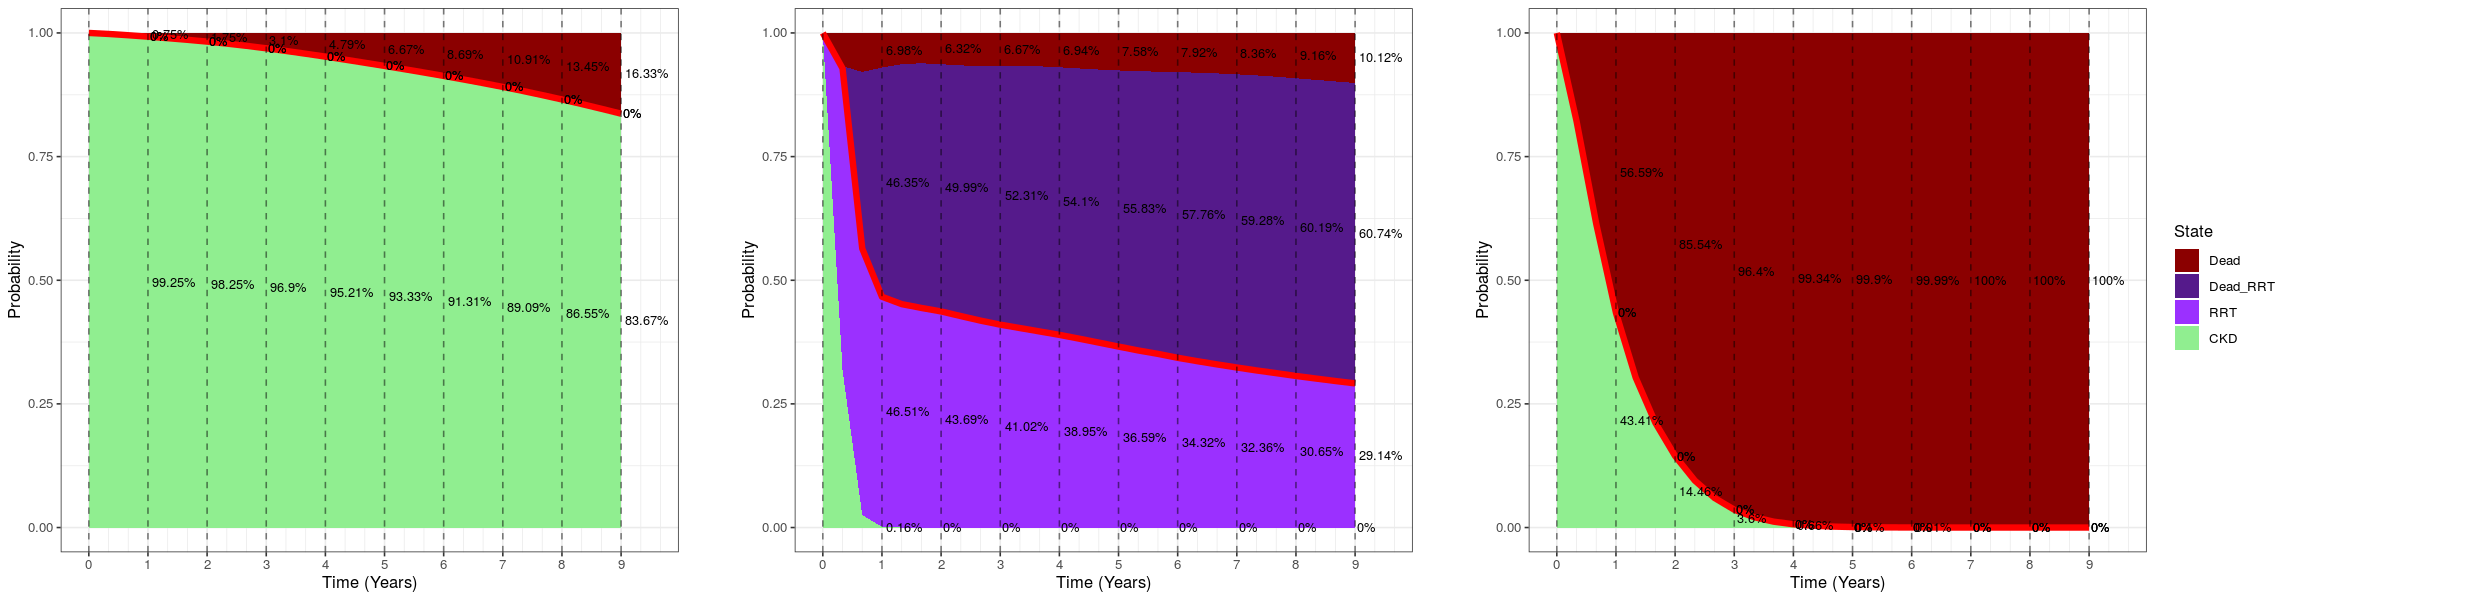
\includegraphics[width=0.9\linewidth]{figure/Dev_Paper_Example} \caption{Results of Example Patients}\label{fig:Example-Predictions-trend}
\end{figure}
\hypertarget{calculator-1}{%
\subsection{Calculator}\label{calculator-1}}

The calculator is available online here:

\url{https://michael-barrowman.shinyapps.io/MSCPM_for_CKD_Patients/}.

\hypertarget{discussion}{%
\section{Discussion}\label{discussion}}

We have used data provided by SKS to develop a Multi-State Clinical Prediction Model and then validated this model within the SKS and SERPR datasets. Within our Models, the cause of a patient's renal disease had the widest effect on patient outcomes meaning that outcomes are highly dependent on ERA-EDTA classification of the diagnosis. Most groupings resulted in a lowered hazard of death and an increased hazard of RRT compared to the baseline of Systemic diseases.

Models performed well in model validation with the Three-State Model slightly out performing the other two models in calibration and overall predictive ability, however the Five-State model performed marginally better in terms of discriminative ability. Both Multi-State Models outperformed the Two-State (Traditional) Model.

The application of a Multi-state clinical prediction model to this field is novel and gives a powerful tool for providing individualised predictions of multiple outcomes at a wide range of time points. The general inclusion criteria for the development dataset, and the wide range of patient ages and measurements allows for the model to be applied to a broad spectrum of patients.

Although the inclusion criteria for SKS were broad, the demographics of the local area resulted in homogeneity of ethnicity, which may create a limitation to the applicability of our model. The Renal Department at SRFT is a tertiary care facility for CKD sufferers and is well renowned for its capabilities of care meaning that it is likely to attract less-healthy patients from a wider catchment area, making the cohort of patients in the development population in worse condition than the general population of CKD patients.

There were also high levels of missingness in the eGFR and uPCR rates of changes would also produce a bias, due to these measures likely being missing not at random. The derivation of the validation dataset ensured that all patients had an eGFR Rate measurement; this was done to avoid data missing not at random (only negative or missing data would be available as patient's eGFR dropped to less than 60), however deriving data in this way could itself induce a survivor bias in the start date used for patients.

In the Five-State Model, We omitted the analysis of the Tx to Dead state due to the anticipated low number of events within the SKS dataset. The lowest number of events for a transition was therefore PD to Dead, which had only 107. Altogether, we considered 26 covariates (with 4 categorical covariates) and so this equates to 36 predictor parameters and an events per predictor parameter (EPP) of 2.97. This is below the recommendations of Riley et al {[}\protect\hyperlink{ref-riley_minimum_2019}{67}{]}, whose calculations produce a requirement of 4.54 EPP. This requirement was also not satisfied by the CKD to PD transition (EPP = 6.36,required = 10.2) or the CKD to Tx transition (EPP = 2.97, required = 17.6). Fortunately, this limitation is confined to the Five-State Model.

We have assumed a proportional hazards relationship between the predictors and probability of survival, which is considered by some to be a strong assumption to make, however we acknowledge this limitation, and the authors believe that it is mitigated by the flexibility that the assumption permits. In addition to the general PH assumption, the R-P model requires the assumption that the log cumulative hazard function follows a cubic spline, (however this is a much weaker assumption {[}\protect\hyperlink{ref-royston_flexible_2002}{68}{]}), which is modelled as part of the regression. We did not assess the viability of these models as it was believed this assumption to make our results more understandable.

Compared to the raw internal validation, the model performance during the external validation was worse for all metrics. However, once adjusted for optimism, the results were much more cohesive which implies that the model is highly transportable to a new population without much alterations being required. Due to the differences in the healthcare systems of England and Scotland, it can be appreciated that despite the populations being similar, their care would be different enough to emphasise a larger difference between our populations than that shown in our (relatively homogeneous) populations.

Although not directly assessing causality in regards to state-transitions, our Three-State model can be used by clinicians to either expedite or delay transition of a patient onto RRT, if it is believed that this would be beneficial. Alternatively, the Five-State Model can be interpreted to provide information regarding \emph{which} treatment might be benficial for a patient.

Our paper has clearly demonstrated the accuracy of such a model. However, further research would be needed to establish the effectiveness and efficacy of its use in clinical practice {[}\protect\hyperlink{ref-moons_prognosis_2009-1}{69}{]} by comparing it to standard care and establishing whether the use of our model improves patient outcomes.

All three models produced for this work performed well in terms of accuracy, calibration and discrimination when applied internally and externally. This shows directly that the models are suitable for use in populations similar to both our development and our validation datasets. It can also be concluded that the models can be transported and applied to any population with a similar healthcare system to the UK.

\hypertarget{appendix-appendices}{%
\appendix}


\hypertarget{chap-dev-paper-supp}{%
\chapter{Development and External Validation of a Multi-State Clinical Prediction Model for Chronic Kidney Disease Patients Progressing onto Renal Replacement Therapy and Death - Supplementary Material}\label{chap-dev-paper-supp}}

\hypertarget{statistical-analysis}{%
\section{Statistical Analysis}\label{statistical-analysis}}

\hypertarget{development}{%
\subsection{Development}\label{development}}

Data was recorded in a time-updated manner, however all variables were measured at baseline to emulate the real-world application of the model (i.e.~future prediction of states and not covariates). Variables considered as covariates were demographics (sex, age, smoking status and alcohol consumption), comorbidities (congestive cardiac failure (CCF), chronic obstructive pulmonary disease (COPD), prior cerebrovascular accident (CVA), hypertension (HT), diabetes mellitus (DM), ischemic heart disease (IHD), chronic liver disease (LD), prior myocardial infarction (MI), peripheral vascular disease (PVD) and slid tumour (ST)), physical parameters (BMI, blood pressure), blood results (haemoglobin, albumin, corrected calcium and phosphate measures), urine protein creatinine ratio (uPCR) and primary renal diagnosis (grouped as per ERA-EDTA classifications {[}\protect\hyperlink{ref-venkat-raman_new_2012}{70}{]}). Ethnicity was assessed in the populations, but as most patients were white, it was omitted as a potential predictor from the models.

uPCR and eGFR Rate of change were also calculated {[}\protect\hyperlink{ref-kovesdy_past_2016}{71}{]}, {[}\protect\hyperlink{ref-naimark_past_2016}{72}{]} as the difference between the two most recent measures divided by time difference in years. \(\textrm{Age}^2\), log(Age), log(eGFR Rate) and log(uPCR Rate) were considered as transformations within the model. log(Calendar Time) was included as a covariate to adjust for time trends in treatment preferences {[}\textbf{Cite: Something}{]}. Calendar Time was defined as length of time between start date and 1st January 2019. {[}\textbf{Matt mentioned the use of log Calendar Time rather than simply Calendar Time. I read this a while ago and can't currently locate the paper (I believe it was a simulation study). I'll carry on looking for it though of course}{]}

Intermediate states (RRT or modality) were considered to be medically transformative, and so a semi-markov (clock reset) method for analysis was considered to be well justified {[}\protect\hyperlink{ref-meira-machado_multi-state_2009}{73}{]}. Each transition was modelled under a proportional hazards assumption using the Royston-Parmar technique {[}\protect\hyperlink{ref-royston_flexible_2002}{68}{]} to estimate coefficients for each covariate and a restricted cubic spline (on the log-time scale) for the baseline cumulative hazard. The cumulative hazards for each transition can be combined to produce estimates for the probability of a patient being in any state at any time {[}\protect\hyperlink{ref-putter_tutorial_2007}{74}{]}.

For variable selection, we stacked the imputed datasets together to create a larger, pseudo-population {[}\protect\hyperlink{ref-wood_how_2008}{75}{]} and performed backwards-forwards selection based on minimising the AIC at each step. This was repeated for each transition and for different numbers of evenly spaced knots in modelling the form of the baseline hazard, K=\{0,1,2,3,4,5\}. This allowed for different transitions to use different sets of variables and numbers of knots in the final model. Some combinations of variables resulted in models that were intractable and so these models were excluded. Once a set of variables were chosen, the R-P model was applied to each imputed dataset individually and the resulting coefficients and cubic spline parameters were aggregated across imputations using Rubin's Rules {[}\protect\hyperlink{ref-rubin_multiple_1984}{76}{]}. This gave a model fully defined by smooth cubic splines representing the cumulative cause-specific hazard and individualised proportional hazards for each transition.

All missing data were assumed to be missing at random and so were multiply imputed using chained equations with the Nelson-Aalen estimators for each relevant transition as predictors {[}\protect\hyperlink{ref-white_imputing_2009}{77}{]}. Some variables (smoking status and histories of COPD, LD and ST) were present in the SKS (development) dataset, but were completely missing in the SERPR extract (validation) and so these were multiply imputed from the development dataset {[}\protect\hyperlink{ref-janssen_dealing_2009}{78}{]}.

\hypertarget{validation}{%
\subsection{Validation}\label{validation}}

Further to the simple individual validation performed above. A statistical validation will need to be performed to formally establish the performance of the models.

Each of the three models were internally validated in the development dataset using bootstrapping to adjust for optimism and then further externally validated in the validation dataset extracted from SERPR{[}\protect\hyperlink{ref-schomaker_bootstrap_2018}{79}{]}. The bootstrapping method was also used for both validations to produce confidence intervals around the performance metric estimates.. To assess the performance in low eGFR patients, the models were also validated in subsets of the SKS and SERPR where patients had an \(\textrm{eGFR} < 30\textrm{ml}/\textrm{min}/1.73\textrm{m}^2\).

For validation purposes, we consider Death and Death after RRT/HD/PD to be distinct states meaning that for the Three-State model, we have \(K=4\) pathways a patient can take and for the Five-State model, we have \(K=7\). To compare across models, we combined states together to collapse down to simpler versions. We collapsed the Three-State model to a two-state structure by combining the CKD and RRT states into an Alive state. We collapsed the Five-State model to a three-state structure by combining the HD, PD and Tx into an RRT state and then further down to a two-state structure as with the Three-State model. We will report performance measures at 360 days (approx. 1-year), 720 days (approx. 2-years) and 1800 days (approx. 5-years). As well as presenting the performance measures over time.

The performance metrics were chosen from those defined in chapter \{\#chap-performance-metrics\}.

The overall accuracy of each model was assessed using the MSM adjusted Brier Scoreas defined in , which is a proper score function assigning 0 to a non-informative model and 1 to a perfect model, with negative numbers implying the model performs worse than assuming every patient's state predictions are the same as the overall prevalence within the population.

The discrimination of each model was assessed using the MSM extension to the c-statistic {[}\protect\hyperlink{ref-calster_extending_2012-1}{80}{]}. The c-statistic is a score between 0 and 1 with higher scores suggesting a better model and a c-statistic of 0.5 suggesting the model performs no better than a non-informative model.

The calibration of each model was assessed using MSM multinomial logistic regression (MLR) {[}\protect\hyperlink{ref-hoorde_assessing_2014}{81}{]} which extends the logistic regression to three or more mutually exclusive outcomes {[}\protect\hyperlink{ref-riley_prognosis_2019}{82}{]}. This produces an intercept vector of length \(K-1\) and a Slope-matrix of dimension \((K-1) \times (K-1)\). As with the traditional calibration intercept for a well performing model, the MLR intercept values should all be as close to 0 as possible. The traditional calibration slope should be as close to 1 as possible and so the multi-state extension of the slope, the Slope-matrix should be as close to the identity matrix (\(I\)) as possible.

\hypertarget{model-results}{%
\section{Model Results}\label{model-results}}

{[}\textbf{Describe the model results briefly}{]}

\hypertarget{two-state-model}{%
\subsection{Two State Model}\label{two-state-model}}

Table \ref{tab:PH-Two} shows the proportional hazard ratios for the transitions in the Two-State Model.
\begin{table}[!h]

\caption{\label{tab:PH-Two}{\small Proportional Hazards for each transition in the Two-State Model}}
\centering
\fontsize{7}{9}\selectfont
\begin{tabular}[t]{l>{\raggedleft\arraybackslash}p{3cm}}
\toprule
  & Alive to Dead\\
\midrule
\rowcolor{gray!6}  \addlinespace[0.3em]
\multicolumn{2}{l}{\textbf{Age}}\\
\hspace{1em}(Age-60) & 0.110 (  -0.055,   0.275)\\
\hspace{1em}(Age-60)\textsuperscript{2} & -0.000 (  -0.001,   0.000)\\
\rowcolor{gray!6}  \hspace{1em}log(Age) & -2.853 ( -12.306,   6.599)\\
\addlinespace[0.3em]
\multicolumn{2}{l}{\textbf{eGFR}}\\
\hspace{1em}eGFR & -0.013 (  -0.018,  -0.008)\\
\rowcolor{gray!6}  \hspace{1em}eGFR Rate & -0.007 (  -0.090,   0.075)\\
\hspace{1em}log(eGFR Rate) & 0.090 (  -0.199,   0.380)\\
\rowcolor{gray!6}  \addlinespace[0.3em]
\multicolumn{2}{l}{\textbf{uPCR}}\\
\hspace{1em}uPCR & \\
\hspace{1em}uPCR Rate & \\
\rowcolor{gray!6}  \hspace{1em}log(uPCR Rate) & \\
\addlinespace[0.3em]
\multicolumn{2}{l}{\textbf{Measures}}\\
\hspace{1em}SBP & \\
\rowcolor{gray!6}  \hspace{1em}DBP & 0.004 (  -0.000,   0.009)\\
\hspace{1em}BMI & \\
\rowcolor{gray!6}  \hspace{1em}Albumin & -0.048 (  -0.061,  -0.034)\\
\hspace{1em}Corrected Calcium & 0.222 (  -0.153,   0.599)\\
\rowcolor{gray!6}  \hspace{1em}Haemoglobin & -0.011 (  -0.015,  -0.007)\\
\hspace{1em}Phosphate & 0.338 (   0.119,   0.557)\\
\rowcolor{gray!6}  \addlinespace[0.3em]
\multicolumn{2}{l}{\textbf{Gender}}\\
\hspace{1em}Female & -0.172 (  -0.291,  -0.053)\\
\addlinespace[0.3em]
\multicolumn{2}{l}{\textbf{Smoking Status}}\\
\hspace{1em}Former (3 years+) & -0.403 (  -0.908,   0.101)\\
\rowcolor{gray!6}  \hspace{1em}Non-Smoker & -0.226 (  -0.358,  -0.095)\\
\hspace{1em}Smoker & 0.376 (   0.212,   0.539)\\
\rowcolor{gray!6}  \addlinespace[0.3em]
\multicolumn{2}{l}{\textbf{Primary Renal Diagnosis}}\\
\hspace{1em}Familial / hereditary nephropathies & -0.399 (  -0.728,  -0.070)\\
\hspace{1em}Glomerular disease & -0.406 (  -0.618,  -0.193)\\
\rowcolor{gray!6}  \hspace{1em}Miscellaneous renal disorders & -0.220 (  -0.434,  -0.005)\\
\hspace{1em}Tubulointerstitial disease & -0.452 (  -0.696,  -0.208)\\
\rowcolor{gray!6}  \addlinespace[0.3em]
\multicolumn{2}{l}{\textbf{Comorbidity}}\\
\hspace{1em}DM & 0.144 (   0.022,   0.265)\\
\hspace{1em}CCF & -0.378 (  -0.505,  -0.252)\\
\rowcolor{gray!6}  \hspace{1em}MI & -0.165 (  -0.304,  -0.026)\\
\hspace{1em}IHD & 0.070 (  -0.059,   0.200)\\
\rowcolor{gray!6}  \hspace{1em}PVD & -0.240 (  -0.371,  -0.109)\\
\hspace{1em}CVA & -0.128 (  -0.293,   0.036)\\
\rowcolor{gray!6}  \hspace{1em}COPD & -0.203 (  -0.330,  -0.076)\\
\hspace{1em}LD & -0.241 (  -0.573,   0.091)\\
\rowcolor{gray!6}  \hspace{1em}ST & -0.299 (  -0.440,  -0.158)\\
\hspace{1em}HT & -0.080 (  -0.339,   0.177)\\
\bottomrule
\end{tabular}
\end{table}
Table \ref{tab:Hazard-Two} shows the hazard functions for the transitions in the Two-State Model.

Table \ref{tab:IV-Two} shows the results from the internal validation in the Two-State Model.

Table \ref{tab:EV-Two} shows the results from the external validation in the Two-State Model.

\hypertarget{three-state-model}{%
\subsection{Three State Model}\label{three-state-model}}

In the Three-State Model, older patients are predicted to be likely to transition to RRT. Increased rates of decline of eGFR were associated with the transition from CKD to RRT. The full results are shown in table \ref{tab:PH-Three}.
\begin{landscape}\begin{table}

\caption{\label{tab:PH-Three}{\small Proportional Hazards for each transition in the Three-State Model}}
\centering
\fontsize{7}{9}\selectfont
\begin{tabular}[t]{l>{\raggedleft\arraybackslash}p{3cm}>{\raggedleft\arraybackslash}p{3cm}>{\raggedleft\arraybackslash}p{3cm}}
\toprule
  & CKD to Dead & CKD to RRT & RRT to Dead\\
\midrule
\rowcolor{gray!6}  \addlinespace[0.3em]
\multicolumn{4}{l}{\textbf{Age}}\\
\hspace{1em}(Age-60) & 0.161 (  -0.051,   0.374) & -0.041 (  -0.051,  -0.031) & 0.063 (   0.050,   0.076)\\
\hspace{1em}(Age-60)\textsuperscript{2} & -0.000 (  -0.002,   0.000) & -0.000 (  -0.000,  -0.000) & \\
\rowcolor{gray!6}  \hspace{1em}log(Age) & -5.725 ( -17.969,   6.518) &  & \\
\addlinespace[0.3em]
\multicolumn{4}{l}{\textbf{eGFR}}\\
\hspace{1em}eGFR & -0.013 (  -0.019,  -0.006) & -0.095 (  -0.108,  -0.082) & 0.011 (  -0.001,   0.025)\\
\rowcolor{gray!6}  \hspace{1em}eGFR Rate &  & 0.055 (  -0.021,   0.131) & -0.056 (  -0.363,   0.250)\\
\hspace{1em}log(eGFR Rate) & 0.042 (  -0.125,   0.210) &  & 0.227 (  -0.770,   1.225)\\
\rowcolor{gray!6}  \addlinespace[0.3em]
\multicolumn{4}{l}{\textbf{uPCR}}\\
\hspace{1em}uPCR & 0.125 (  -0.318,   0.569) & 0.700 (   0.112,   1.288) & -0.108 (  -0.736,   0.519)\\
\hspace{1em}uPCR Rate &  & -0.019 (  -0.045,   0.005) & 0.036 (  -0.062,   0.136)\\
\rowcolor{gray!6}  \hspace{1em}log(uPCR Rate) &  & 0.218 (  -0.310,   0.747) & -0.198 (  -0.534,   0.137)\\
\addlinespace[0.3em]
\multicolumn{4}{l}{\textbf{Measures}}\\
\hspace{1em}SBP & -0.001 (  -0.004,   0.002) & 0.005 (  -0.000,   0.011) & \\
\rowcolor{gray!6}  \hspace{1em}DBP & 0.006 (   0.000,   0.013) & 0.006 (  -0.001,   0.015) & \\
\hspace{1em}BMI &  &  & \\
\rowcolor{gray!6}  \hspace{1em}Albumin & -0.044 (  -0.064,  -0.024) & -0.032 (  -0.059,  -0.004) & -0.044 (  -0.079,  -0.009)\\
\hspace{1em}Corrected Calcium & 0.280 (  -0.192,   0.752) & -0.515 (  -1.207,   0.177) & \\
\rowcolor{gray!6}  \hspace{1em}Haemoglobin & -0.013 (  -0.017,  -0.008) & -0.005 (  -0.012,   0.001) & -0.005 (  -0.014,   0.003)\\
\hspace{1em}Phosphate & 0.511 (   0.132,   0.890) & 0.869 (  -0.059,   1.799) & \\
\rowcolor{gray!6}  \addlinespace[0.3em]
\multicolumn{4}{l}{\textbf{Gender}}\\
\hspace{1em}Female & -0.235 (  -0.371,  -0.099) & -0.277 (  -0.455,  -0.099) & \\
\addlinespace[0.3em]
\multicolumn{4}{l}{\textbf{Smoking Status}}\\
\hspace{1em}Former (3 years+) & -0.212 (  -0.879,   0.453) & -0.133 (  -0.757,   0.490) & -0.282 (  -1.082,   0.518)\\
\rowcolor{gray!6}  \hspace{1em}Non-Smoker & -0.198 (  -0.345,  -0.051) & -0.162 (  -0.364,   0.039) & -0.294 (  -0.598,   0.009)\\
\hspace{1em}Smoker & 0.356 (   0.160,   0.551) & 0.175 (  -0.076,   0.428) & 0.387 (   0.068,   0.706)\\
\rowcolor{gray!6}  \addlinespace[0.3em]
\multicolumn{4}{l}{\textbf{Primary Renal Diagnosis}}\\
\hspace{1em}Familial / hereditary nephropathies & -0.424 (  -0.854,   0.006) & 1.029 (   0.720,   1.338) & -0.562 (  -1.084,  -0.040)\\
\hspace{1em}Glomerular disease & -0.394 (  -0.635,  -0.154) & -0.165 (  -0.465,   0.134) & -0.488 (  -0.883,  -0.094)\\
\rowcolor{gray!6}  \hspace{1em}Miscellaneous renal disorders & -0.263 (  -0.505,  -0.021) & -0.649 (  -1.143,  -0.155) & 0.033 (  -0.553,   0.620)\\
\hspace{1em}Tubulointerstitial disease & -0.463 (  -0.741,  -0.184) & -0.265 (  -0.577,   0.046) & -0.310 (  -0.803,   0.181)\\
\rowcolor{gray!6}  \addlinespace[0.3em]
\multicolumn{4}{l}{\textbf{Comorbidity}}\\
\hspace{1em}DM & 0.122 (  -0.011,   0.255) & 0.141 (  -0.074,   0.358) & 0.200 (  -0.096,   0.496)\\
\hspace{1em}CCF & -0.394 (  -0.535,  -0.253) &  & -0.299 (  -0.597,  -0.002)\\
\rowcolor{gray!6}  \hspace{1em}MI & -0.246 (  -0.397,  -0.094) & 0.234 (  -0.061,   0.530) & 0.186 (  -0.199,   0.572)\\
\hspace{1em}IHD & 0.102 (  -0.041,   0.245) & -0.077 (  -0.334,   0.179) & -0.097 (  -0.424,   0.228)\\
\rowcolor{gray!6}  \hspace{1em}PVD & -0.248 (  -0.394,  -0.103) & -0.168 (  -0.405,   0.068) & -0.183 (  -0.492,   0.126)\\
\hspace{1em}CVA & -0.070 (  -0.252,   0.111) &  & -0.168 (  -0.577,   0.240)\\
\rowcolor{gray!6}  \hspace{1em}COPD & -0.289 (  -0.433,  -0.145) &  & \\
\hspace{1em}LD & -0.169 (  -0.578,   0.239) & -0.316 (  -0.731,   0.097) & -0.270 (  -0.858,   0.318)\\
\rowcolor{gray!6}  \hspace{1em}ST & -0.274 (  -0.431,  -0.117) & -0.181 (  -0.516,   0.153) & -0.278 (  -0.611,   0.055)\\
\hspace{1em}HT &  & 0.274 (  -0.176,   0.726) & -0.416 (  -1.104,   0.271)\\
\bottomrule
\end{tabular}
\end{table}
\end{landscape}
Female patients are predicted to be more likely to remain in the CKD state than Males, or to remain in the RRT state once there. Smokers were predicted as more likely than Non-/Former Smokers to undergo any transition, apart from CKD to Tx. Blood results had associations with all transitions in some way, and disease etiology were strongly associated with the transitions giving a wide range of predictions.

Table \ref{tab:Hazard-Three} shows the hazard functions for the transitions in the Three-State Model.

Table \ref{tab:IV-Three} shows the results from the internal validation in the Three-State Model.

Table \ref{tab:EV-Three} shows the results from the external validation in the Three-State Model.

\hypertarget{five-state-model}{%
\subsection{Five State Model}\label{five-state-model}}

Table \ref{tab:PH-Five} shows the proportional hazard ratios for the transitions in the Five-State Model.
\begin{landscape}\begin{table}

\caption{\label{tab:PH-Five}{\small Proportional Hazards for each transition in the Five-State Model}}
\centering
\fontsize{7}{9}\selectfont
\begin{tabular}[t]{l>{\raggedleft\arraybackslash}p{3cm}>{\raggedleft\arraybackslash}p{3cm}>{\raggedleft\arraybackslash}p{3cm}>{\raggedleft\arraybackslash}p{3cm}>{\raggedleft\arraybackslash}p{3cm}>{\raggedleft\arraybackslash}p{3cm}}
\toprule
  & CKD to Dead & CKD to HD & CKD to PD & CKD to Tx & HD to Dead & PD to Dead\\
\midrule
\rowcolor{gray!6}  \addlinespace[0.3em]
\multicolumn{7}{l}{\textbf{Age}}\\
\hspace{1em}(Age-60) & 0.161 (  -0.051,   0.374) & -0.029 (  -0.047,  -0.011) & -0.037 (  -0.057,  -0.018) & -0.099 (  -0.127,  -0.072) & 0.069 (   0.051,   0.087) & 0.046 (   0.024,   0.068)\\
\hspace{1em}(Age-60)\textsuperscript{2} & -0.000 (  -0.002,   0.000) & -0.000 (  -0.001,   0.000) & -0.000 (  -0.000,   0.000) & -0.000 (  -0.001,  -0.000) &  & \\
\rowcolor{gray!6}  \hspace{1em}log(Age) & -5.725 ( -17.969,   6.518) &  &  &  &  & \\
\addlinespace[0.3em]
\multicolumn{7}{l}{\textbf{eGFR}}\\
\hspace{1em}eGFR & -0.013 (  -0.019,  -0.006) & -0.088 (  -0.105,  -0.071) & -0.112 (  -0.135,  -0.090) & -0.097 (  -0.120,  -0.074) & 0.016 (   0.000,   0.032) & -0.006 (  -0.036,   0.023)\\
\rowcolor{gray!6}  \hspace{1em}eGFR Rate &  & 0.085 (  -0.058,   0.229) &  & -0.169 (  -0.813,   0.474) & -0.053 (  -0.701,   0.593) & 0.000 (  -0.294,   0.294)\\
\hspace{1em}log(eGFR Rate) & 0.042 (  -0.125,   0.210) & -0.261 (  -0.798,   0.276) & 0.445 (  -0.280,   1.171) & 0.440 (  -1.371,   2.252) & 0.366 (  -1.344,   2.077) & \\
\rowcolor{gray!6}  \addlinespace[0.3em]
\multicolumn{7}{l}{\textbf{uPCR}}\\
\hspace{1em}uPCR & 0.125 (  -0.318,   0.569) & 0.738 (   0.024,   1.451) & 0.650 (  -0.906,   2.207) & 0.317 (  -0.606,   1.241) & -0.577 (  -1.317,   0.162) & 0.071 (  -1.109,   1.251)\\
\hspace{1em}uPCR Rate &  &  & -0.042 (  -0.139,   0.055) & 0.020 (  -0.050,   0.091) & 0.030 (  -0.039,   0.099) & \\
\rowcolor{gray!6}  \hspace{1em}log(uPCR Rate) &  & -0.097 (  -0.880,   0.685) & 0.740 (  -0.470,   1.950) & -0.244 (  -0.940,   0.450) &  & -0.080 (  -0.515,   0.354)\\
\addlinespace[0.3em]
\multicolumn{7}{l}{\textbf{Measures}}\\
\hspace{1em}SBP & -0.001 (  -0.004,   0.002) & 0.003 (  -0.003,   0.010) & 0.009 (  -0.001,   0.020) &  &  & \\
\rowcolor{gray!6}  \hspace{1em}DBP & 0.006 (   0.000,   0.013) & 0.007 (  -0.005,   0.021) & 0.007 (  -0.010,   0.025) &  &  & \\
\hspace{1em}BMI &  & 0.003 (  -0.063,   0.070) &  & -0.019 (  -0.060,   0.021) &  & \\
\rowcolor{gray!6}  \hspace{1em}Albumin & -0.044 (  -0.064,  -0.024) & -0.040 (  -0.075,  -0.005) & -0.037 (  -0.100,   0.025) &  & -0.050 (  -0.096,  -0.003) & -0.021 (  -0.076,   0.032)\\
\hspace{1em}Corrected Calcium & 0.280 (  -0.192,   0.752) &  & -1.291 (  -2.494,  -0.089) &  &  & 1.243 (  -0.187,   2.674)\\
\rowcolor{gray!6}  \hspace{1em}Haemoglobin & -0.013 (  -0.017,  -0.008) & -0.009 (  -0.018,  -0.000) & -0.001 (  -0.016,   0.013) & -0.003 (  -0.016,   0.010) & -0.006 (  -0.017,   0.005) & -0.022 (  -0.037,  -0.006)\\
\hspace{1em}Phosphate & 0.511 (   0.132,   0.890) & 0.904 (   0.087,   1.721) & 1.042 (  -0.336,   2.421) & 0.578 (  -0.333,   1.491) &  & \\
\rowcolor{gray!6}  \addlinespace[0.3em]
\multicolumn{7}{l}{\textbf{Gender}}\\
\hspace{1em}Female & -0.235 (  -0.371,  -0.099) & -0.492 (  -0.754,  -0.230) & -0.156 (  -0.466,   0.154) &  &  & \\
\addlinespace[0.3em]
\multicolumn{7}{l}{\textbf{Smoking Status}}\\
\hspace{1em}Former (3 years+) & -0.212 (  -0.879,   0.453) & -0.121 (  -1.020,   0.776) & -0.337 (  -1.527,   0.851) & 0.599 (  -0.501,   1.701) & -0.519 (  -1.745,   0.706) & -0.026 (  -1.302,   1.249)\\
\rowcolor{gray!6}  \hspace{1em}Non-Smoker & -0.198 (  -0.345,  -0.051) & -0.168 (  -0.567,   0.230) & -0.056 (  -0.405,   0.291) & -0.161 (  -0.623,   0.299) & -0.192 (  -0.641,   0.256) & -0.481 (  -1.013,   0.049)\\
\hspace{1em}Smoker & 0.356 (   0.160,   0.551) & 0.259 (  -0.091,   0.611) & 0.374 (  -0.004,   0.753) & -0.532 (  -1.202,   0.136) & 0.686 (   0.252,   1.120) & 0.136 (  -0.400,   0.674)\\
\rowcolor{gray!6}  \addlinespace[0.3em]
\multicolumn{7}{l}{\textbf{Primary Renal Diagnosis}}\\
\hspace{1em}Familial / hereditary nephropathies & -0.424 (  -0.854,   0.006) & 0.869 (   0.391,   1.348) & 0.982 (   0.466,   1.498) & 1.330 (   0.504,   2.156) & -0.775 (  -1.444,  -0.105) & -0.397 (  -1.214,   0.419)\\
\hspace{1em}Glomerular disease & -0.394 (  -0.635,  -0.154) & -0.313 (  -0.716,   0.090) & -0.263 (  -0.706,   0.178) & 0.224 (  -0.349,   0.797) & -0.683 (  -1.146,  -0.221) & -0.332 (  -0.994,   0.330)\\
\rowcolor{gray!6}  \hspace{1em}Miscellaneous renal disorders & -0.263 (  -0.505,  -0.021) & -0.375 (  -0.927,   0.176) & -1.319 (  -2.390,  -0.247) & -1.377 (  -2.859,   0.103) & -0.364 (  -1.039,   0.310) & 0.999 (  -0.340,   2.338)\\
\hspace{1em}Tubulointerstitial disease & -0.463 (  -0.741,  -0.184) & -0.307 (  -0.788,   0.173) & -0.311 (  -0.904,   0.281) & -0.232 (  -1.130,   0.666) & -0.599 (  -1.247,   0.048) & 0.428 (  -0.427,   1.284)\\
\rowcolor{gray!6}  \addlinespace[0.3em]
\multicolumn{7}{l}{\textbf{Comorbidity}}\\
\hspace{1em}DM & 0.122 (  -0.011,   0.255) & 0.123 (  -0.187,   0.434) &  &  &  & 0.570 (   0.017,   1.124)\\
\hspace{1em}CCF & -0.394 (  -0.535,  -0.253) & -0.144 (  -0.517,   0.228) & 0.378 (  -0.094,   0.852) & 0.341 (  -0.529,   1.213) & -0.174 (  -0.576,   0.228) & -0.389 (  -0.994,   0.216)\\
\rowcolor{gray!6}  \hspace{1em}MI & -0.246 (  -0.397,  -0.094) &  & 0.274 (  -0.313,   0.862) & 1.602 (  -0.445,   3.650) & 0.304 (  -0.152,   0.761) & \\
\hspace{1em}IHD & 0.102 (  -0.041,   0.245) &  & -0.440 (  -0.869,  -0.010) & 0.864 (  -0.634,   2.362) &  & -0.236 (  -0.852,   0.378)\\
\rowcolor{gray!6}  \hspace{1em}PVD & -0.248 (  -0.394,  -0.103) &  & -0.203 (  -0.631,   0.224) & -0.600 (  -1.318,   0.118) & -0.315 (  -0.697,   0.067) & \\
\hspace{1em}CVA & -0.070 (  -0.252,   0.111) &  &  & -0.287 (  -1.243,   0.668) &  & -0.833 (  -1.634,  -0.032)\\
\rowcolor{gray!6}  \hspace{1em}COPD & -0.289 (  -0.433,  -0.145) &  & -0.204 (  -0.563,   0.153) & 0.625 (  -0.101,   1.351) & 0.208 (  -0.189,   0.606) & \\
\hspace{1em}LD & -0.169 (  -0.578,   0.239) & -0.659 (  -1.157,  -0.160) & -0.320 (  -1.015,   0.373) & 12.426 (-521.602, 546.454) &  & -0.751 (  -1.941,   0.438)\\
\rowcolor{gray!6}  \hspace{1em}ST & -0.274 (  -0.431,  -0.117) & -0.335 (  -0.777,   0.106) &  &  & -0.184 (  -0.592,   0.223) & -0.419 (  -1.146,   0.306)\\
\hspace{1em}HT &  & 0.139 (  -0.425,   0.705) & 0.447 (  -0.535,   1.429) & 0.458 (  -0.527,   1.443) &  & -0.920 (  -2.113,   0.271)\\
\bottomrule
\end{tabular}
\end{table}
\end{landscape}
Table \ref{tab:Hazard-Five} shows the hazard functions for the transitions in the Five-State Model.

Table \ref{tab:IV-Five} shows the results from the internal validation in the Five-State Model.

Table \ref{tab:EV-Five} shows the results from the external validation in the Five-State Model.

\backmatter

\hypertarget{references}{%
\chapter*{References}\label{references}}
\addcontentsline{toc}{chapter}{References}

\markboth{References}{References}

\noindent

\setlength{\parindent}{-0.20in}
\setlength{\leftskip}{0.20in}
\setlength{\parskip}{8pt}

\hypertarget{refs}{}
\begin{cslreferences}
\leavevmode\hypertarget{ref-steyerberg_prognosis_2013}{}%
{[}1{]} E. W. Steyerberg \emph{et al.}, ``Prognosis Research Strategy (PROGRESS) 3: Prognostic Model Research,'' \emph{PLOS Medicine}, vol. 10, no. 2, p. e1001381, Feb. 2013, doi: \href{https://doi.org/10.1371/journal.pmed.1001381}{10.1371/journal.pmed.1001381}.

\leavevmode\hypertarget{ref-hippisley-cox_development_2017}{}%
{[}2{]} J. Hippisley-Cox, C. Coupland, and P. Brindle, ``Development and validation of QRISK3 risk prediction algorithms to estimate future risk of cardiovascular disease: Prospective cohort study,'' \emph{BMJ}, vol. 357, May 2017, doi: \href{https://doi.org/10.1136/bmj.j2099}{10.1136/bmj.j2099}.

\leavevmode\hypertarget{ref-johnson_predicting_2007}{}%
{[}3{]} E. S. Johnson, M. L. Thorp, X. Yang, O. L. Charansonney, and D. H. Smith, ``Predicting renal replacement therapy and mortality in CKD,'' \emph{American Journal of Kidney Diseases: The Official Journal of the National Kidney Foundation}, vol. 50, no. 4, pp. 559--565, Oct. 2007, doi: \href{https://doi.org/10.1053/j.ajkd.2007.07.006}{10.1053/j.ajkd.2007.07.006}.

\leavevmode\hypertarget{ref-landray_prediction_2010}{}%
{[}4{]} M. J. Landray \emph{et al.}, ``Prediction of ESRD and death among people with CKD: The Chronic Renal Impairment in Birmingham (CRIB) prospective cohort study,'' \emph{American Journal of Kidney Diseases: The Official Journal of the National Kidney Foundation}, vol. 56, no. 6, pp. 1082--1094, Dec. 2010, doi: \href{https://doi.org/10.1053/j.ajkd.2010.07.016}{10.1053/j.ajkd.2010.07.016}.

\leavevmode\hypertarget{ref-bansal_development_2015}{}%
{[}5{]} N. Bansal \emph{et al.}, ``Development and validation of a model to predict 5-year risk of death without ESRD among older adults with CKD,'' \emph{Clinical journal of the American Society of Nephrology: CJASN}, vol. 10, no. 3, pp. 363--371, Mar. 2015, doi: \href{https://doi.org/10.2215/CJN.04650514}{10.2215/CJN.04650514}.

\leavevmode\hypertarget{ref-marks_looking_2015}{}%
{[}6{]} A. Marks \emph{et al.}, ``Looking to the future: Predicting renal replacement outcomes in a large community cohort with chronic kidney disease,'' \emph{Nephrology, Dialysis, Transplantation: Official Publication of the European Dialysis and Transplant Association - European Renal Association}, vol. 30, no. 9, pp. 1507--1517, Sep. 2015, doi: \href{https://doi.org/10.1093/ndt/gfv089}{10.1093/ndt/gfv089}.

\leavevmode\hypertarget{ref-wick_clinical_2017}{}%
{[}7{]} J. P. Wick \emph{et al.}, ``A Clinical Risk Prediction Tool for 6-Month Mortality After Dialysis Initiation Among Older Adults,'' \emph{American Journal of Kidney Diseases: The Official Journal of the National Kidney Foundation}, vol. 69, no. 5, pp. 568--575, May 2017, doi: \href{https://doi.org/10.1053/j.ajkd.2016.08.035}{10.1053/j.ajkd.2016.08.035}.

\leavevmode\hypertarget{ref-johnson_predicting_2008}{}%
{[}8{]} E. S. Johnson, M. L. Thorp, R. W. Platt, and D. H. Smith, ``Predicting the risk of dialysis and transplant among patients with CKD: A retrospective cohort study,'' \emph{American Journal of Kidney Diseases: The Official Journal of the National Kidney Foundation}, vol. 52, no. 4, pp. 653--660, Oct. 2008, doi: \href{https://doi.org/10.1053/j.ajkd.2008.04.026}{10.1053/j.ajkd.2008.04.026}.

\leavevmode\hypertarget{ref-schroeder_predicting_2017}{}%
{[}9{]} E. B. Schroeder \emph{et al.}, ``Predicting 5-Year Risk of RRT in Stage 3 or 4 CKD: Development and External Validation,'' \emph{Clinical journal of the American Society of Nephrology: CJASN}, vol. 12, no. 1, pp. 87--94, Jun. 2017, doi: \href{https://doi.org/10.2215/CJN.01290216}{10.2215/CJN.01290216}.

\leavevmode\hypertarget{ref-kulkarni_transition_2017}{}%
{[}10{]} S. Kulkarni \emph{et al.}, ``Transition probabilities between changing sensitization levels, waitlist activity status and competing-risk kidney transplant outcomes using multi-state modeling,'' \emph{PLOS ONE}, vol. 12, no. 12, p. e0190277, Dec. 2017, doi: \href{https://doi.org/10.1371/journal.pone.0190277}{10.1371/journal.pone.0190277}.

\leavevmode\hypertarget{ref-floege_development_2015}{}%
{[}11{]} J. Floege \emph{et al.}, ``Development and validation of a predictive mortality risk score from a European hemodialysis cohort,'' \emph{Kidney International}, vol. 87, no. 5, pp. 996--1008, May 2015, doi: \href{https://doi.org/10.1038/ki.2014.419}{10.1038/ki.2014.419}.

\leavevmode\hypertarget{ref-hemke_survival_2013}{}%
{[}12{]} A. C. Hemke, M. B. Heemskerk, M. van Diepen, W. Weimar, F. W. Dekker, and A. J. Hoitsma, ``Survival prognosis after the start of a renal replacement therapy in the Netherlands: A retrospective cohort study,'' \emph{BMC Nephrology}, vol. 14, p. 258, Nov. 2013, doi: \href{https://doi.org/10.1186/1471-2369-14-258}{10.1186/1471-2369-14-258}.

\leavevmode\hypertarget{ref-cao_predicting_2015}{}%
{[}13{]} X.-Y. Cao \emph{et al.}, ``Predicting one-year mortality in peritoneal dialysis patients: An analysis of the China Peritoneal Dialysis Registry,'' \emph{International Journal of Medical Sciences}, vol. 12, no. 4, pp. 354--361, 2015, doi: \href{https://doi.org/10.7150/ijms.11694}{10.7150/ijms.11694}.

\leavevmode\hypertarget{ref-tangri_predictive_2011}{}%
{[}14{]} N. Tangri \emph{et al.}, ``A predictive model for progression of chronic kidney disease to kidney failure,'' \emph{JAMA}, vol. 305, no. 15, pp. 1553--1559, Apr. 2011, doi: \href{https://doi.org/10.1001/jama.2011.451}{10.1001/jama.2011.451}.

\leavevmode\hypertarget{ref-roy_statistical_2017}{}%
{[}15{]} J. Roy \emph{et al.}, ``Statistical Methods for Cohort Studies of CKD: Prediction Modeling,'' \emph{Clinical journal of the American Society of Nephrology: CJASN}, vol. 12, no. 6, pp. 1010--1017, Jun. 2017, doi: \href{https://doi.org/10.2215/CJN.06210616}{10.2215/CJN.06210616}.

\leavevmode\hypertarget{ref-tangri_dynamic_2017}{}%
{[}16{]} N. Tangri \emph{et al.}, ``A Dynamic Predictive Model for Progression of CKD,'' \emph{American Journal of Kidney Diseases: The Official Journal of the National Kidney Foundation}, vol. 69, no. 4, pp. 514--520, Apr. 2017, doi: \href{https://doi.org/10.1053/j.ajkd.2016.07.030}{10.1053/j.ajkd.2016.07.030}.

\leavevmode\hypertarget{ref-shlipak_cardiovascular_2005}{}%
{[}17{]} M. G. Shlipak \emph{et al.}, ``Cardiovascular mortality risk in chronic kidney disease: Comparison of traditional and novel risk factors,'' \emph{JAMA}, vol. 293, no. 14, pp. 1737--1745, Apr. 2005, doi: \href{https://doi.org/10.1001/jama.293.14.1737}{10.1001/jama.293.14.1737}.

\leavevmode\hypertarget{ref-weiner_framingham_2007}{}%
{[}18{]} D. E. Weiner \emph{et al.}, ``The Framingham predictive instrument in chronic kidney disease,'' \emph{Journal of the American College of Cardiology}, vol. 50, no. 3, pp. 217--224, Jul. 2007, doi: \href{https://doi.org/10.1016/j.jacc.2007.03.037}{10.1016/j.jacc.2007.03.037}.

\leavevmode\hypertarget{ref-mcmurray_predictors_2011}{}%
{[}19{]} J. J. V. McMurray \emph{et al.}, ``Predictors of fatal and nonfatal cardiovascular events in patients with type 2 diabetes mellitus, chronic kidney disease, and anemia: An analysis of the Trial to Reduce cardiovascular Events with Aranesp (darbepoetin-alfa) Therapy (TREAT),'' \emph{American Heart Journal}, vol. 162, no. 4, pp. 748--755.e3, Oct. 2011, doi: \href{https://doi.org/10.1016/j.ahj.2011.07.016}{10.1016/j.ahj.2011.07.016}.

\leavevmode\hypertarget{ref-grams_assessing_2013}{}%
{[}20{]} M. E. Grams and J. Coresh, ``Assessing risk in chronic kidney disease: A methodological review,'' \emph{Nature Reviews. Nephrology}, vol. 9, no. 1, pp. 18--25, Jan. 2013, doi: \href{https://doi.org/10.1038/nrneph.2012.248}{10.1038/nrneph.2012.248}.

\leavevmode\hypertarget{ref-tangri_risk_2013}{}%
{[}21{]} N. Tangri \emph{et al.}, ``Risk prediction models for patients with chronic kidney disease: A systematic review,'' \emph{Annals of Internal Medicine}, vol. 158, no. 8, pp. 596--603, Apr. 2013, doi: \href{https://doi.org/10.7326/0003-4819-158-8-201304160-00004}{10.7326/0003-4819-158-8-201304160-00004}.

\leavevmode\hypertarget{ref-ramspek_prediction_2017}{}%
{[}22{]} C. L. Ramspek, P. W. Voskamp, F. J. van Ittersum, R. T. Krediet, F. W. Dekker, and M. van Diepen, ``Prediction models for the mortality risk in chronic dialysis patients: A systematic review and independent external validation study,'' \emph{Clinical Epidemiology}, vol. 9, pp. 451--464, 2017, doi: \href{https://doi.org/10.2147/CLEP.S139748}{10.2147/CLEP.S139748}.

\leavevmode\hypertarget{ref-collins_transparent_2015}{}%
{[}23{]} G. S. Collins, J. B. Reitsma, D. G. Altman, and K. G. Moons, ``Transparent reporting of a multivariable prediction model for individual prognosis or diagnosis (TRIPOD): The TRIPOD Statement,'' \emph{BMC Medicine}, vol. 13, no. 1, p. 1, Jan. 2015, doi: \href{https://doi.org/10.1186/s12916-014-0241-z}{10.1186/s12916-014-0241-z}.

\leavevmode\hypertarget{ref-bouwmeester_reporting_2012-1}{}%
{[}24{]} W. Bouwmeester \emph{et al.}, ``Reporting and Methods in Clinical Prediction Research: A Systematic Review,'' \emph{PLOS Medicine}, vol. 9, no. 5, p. e1001221, May 2012, doi: \href{https://doi.org/10.1371/journal.pmed.1001221}{10.1371/journal.pmed.1001221}.

\leavevmode\hypertarget{ref-perotte_risk_2015}{}%
{[}25{]} A. Perotte, R. Ranganath, J. S. Hirsch, D. Blei, and N. Elhadad, ``Risk prediction for chronic kidney disease progression using heterogeneous electronic health record data and time series analysis,'' \emph{Journal of the American Medical Informatics Association: JAMIA}, vol. 22, no. 4, pp. 872--880, Jul. 2015, doi: \href{https://doi.org/10.1093/jamia/ocv024}{10.1093/jamia/ocv024}.

\leavevmode\hypertarget{ref-begun_identification_2013}{}%
{[}26{]} A. Begun, A. Icks, R. Waldeyer, S. Landwehr, M. Koch, and G. Giani, ``Identification of a multistate continuous-time nonhomogeneous Markov chain model for patients with decreased renal function.'' \emph{Medical decision making : an international journal of the Society for Medical Decision Making}, vol. 33, no. 2, pp. 298--306, Feb. 2013, doi: \href{https://doi.org/10.1177/0272989X12466731}{10.1177/0272989X12466731}.

\leavevmode\hypertarget{ref-allen_chronic_2014}{}%
{[}27{]} A. M. Allen, W. R. Kim, T. M. Therneau, J. J. Larson, J. K. Heimbach, and A. D. Rule, ``Chronic kidney disease and associated mortality after liver transplantation--a time-dependent analysis using measured glomerular filtration rate,'' \emph{Journal of Hepatology}, vol. 61, no. 2, pp. 286--292, Aug. 2014, doi: \href{https://doi.org/10.1016/j.jhep.2014.03.034}{10.1016/j.jhep.2014.03.034}.

\leavevmode\hypertarget{ref-grams_predicting_2018}{}%
{[}28{]} M. E. Grams \emph{et al.}, ``Predicting timing of clinical outcomes in patients~with chronic kidney disease and severely decreased glomerular filtration rate,'' \emph{Kidney International}, vol. 93, no. 6, pp. 1442--1451, Jun. 2018, doi: \href{https://doi.org/10.1016/j.kint.2018.01.009}{10.1016/j.kint.2018.01.009}.

\leavevmode\hypertarget{ref-altman_problems_1994-1}{}%
{[}29{]} D. G. Altman, ``Problems in dichotomizing continuous variables,'' \emph{American Journal of Epidemiology}, vol. 139, no. 4, pp. 442--445, Feb. 1994, doi: \href{https://doi.org/10.1093/oxfordjournals.aje.a117020}{10.1093/oxfordjournals.aje.a117020}.

\leavevmode\hypertarget{ref-altman_dangers_1994-1}{}%
{[}30{]} D. G. Altman, B. Lausen, W. Sauerbrei, and M. Schumacher, ``Dangers of Using `Optimal' Cutpoints in the Evaluation of Prognostic Factors,'' \emph{JNCI: Journal of the National Cancer Institute}, vol. 86, no. 11, pp. 829--835, Jun. 1994, doi: \href{https://doi.org/10.1093/jnci/86.11.829}{10.1093/jnci/86.11.829}.

\leavevmode\hypertarget{ref-altman_cost_2006-1}{}%
{[}31{]} D. G. Altman and P. Royston, ``The cost of dichotomising continuous variables,'' \emph{BMJ}, vol. 332, no. 7549, p. 1080, May 2006, doi: \href{https://doi.org/10.1136/bmj.332.7549.1080}{10.1136/bmj.332.7549.1080}.

\leavevmode\hypertarget{ref-bennette_against_2012-1}{}%
{[}32{]} C. Bennette and A. Vickers, ``Against quantiles: Categorization of continuous variables in epidemiologic research, and its discontents,'' \emph{BMC Medical Research Methodology}, vol. 12, no. 1, p. 21, Feb. 2012, doi: \href{https://doi.org/10.1186/1471-2288-12-21}{10.1186/1471-2288-12-21}.

\leavevmode\hypertarget{ref-butts_chopped_2009-1}{}%
{[}33{]} M. M. Butts and T. W. H. Ng, ``Chopped liver? OK. Chopped data? Not OK,'' in \emph{Statistical and methodological myths and urban legends: Doctrine, verity and fable in the organizational and social sciences}, New York, NY, US: Routledge/Taylor \& Francis Group, 2009, pp. 361--386.

\leavevmode\hypertarget{ref-cumberland_ophthalmic_2014-1}{}%
{[}34{]} P. M. Cumberland \emph{et al.}, ``Ophthalmic statistics note: The perils of dichotomising continuous variables,'' \emph{British Journal of Ophthalmology}, vol. 98, no. 6, pp. 841--843, Jun. 2014, doi: \href{https://doi.org/10.1136/bjophthalmol-2014-304930}{10.1136/bjophthalmol-2014-304930}.

\leavevmode\hypertarget{ref-dawson_dichotomizing_2012-1}{}%
{[}35{]} N. V. Dawson and R. Weiss, ``Dichotomizing continuous variables in statistical analysis: A practice to avoid,'' \emph{Medical Decision Making: An International Journal of the Society for Medical Decision Making}, vol. 32, no. 2, pp. 225--226, doi: \href{https://doi.org/10.1177/0272989X12437605}{10.1177/0272989X12437605}.

\leavevmode\hypertarget{ref-dinero_seven_1996-1}{}%
{[}36{]} T. E. Dinero, ``Seven reasons why you should not categorize continuous data,'' \emph{Journal of Health \& Social Policy}, vol. 8, no. 1, pp. 63--72, 1996, doi: \href{https://doi.org/10.1300/J045v08n01_06}{10.1300/J045v08n01\_06}.

\leavevmode\hypertarget{ref-irwin_negative_2003}{}%
{[}37{]} J. R. Irwin and G. H. McClelland, ``Negative Consequences of Dichotomizing Continuous Predictor Variables,'' \emph{Journal of Marketing Research}, vol. 40, no. 3, pp. 366--371, Aug. 2003, doi: \href{https://doi.org/10.1509/jmkr.40.3.366.19237}{10.1509/jmkr.40.3.366.19237}.

\leavevmode\hypertarget{ref-kuss_danger_2013}{}%
{[}38{]} O. Kuss, ``The danger of dichotomizing continuous variables: A visualization,'' \emph{Teaching Statistics}, vol. 35, no. 2, pp. 78--79, 2013, doi: \href{https://doi.org/10.1111/test.12006}{10.1111/test.12006}.

\leavevmode\hypertarget{ref-metze_dichotomization_2008}{}%
{[}39{]} K. Metze, ``Dichotomization of continuous data--a pitfall in prognostic factor studies,'' \emph{Pathology, Research and Practice}, vol. 204, no. 3, pp. 213--214, 2008, doi: \href{https://doi.org/10.1016/j.prp.2007.12.002}{10.1016/j.prp.2007.12.002}.

\leavevmode\hypertarget{ref-naggara_analysis_2011}{}%
{[}40{]} O. Naggara, J. Raymond, F. Guilbert, D. Roy, A. Weill, and D. G. Altman, ``Analysis by categorizing or dichotomizing continuous variables is inadvisable: An example from the natural history of unruptured aneurysms,'' \emph{AJNR. American journal of neuroradiology}, vol. 32, no. 3, pp. 437--440, Mar. 2011, doi: \href{https://doi.org/10.3174/ajnr.A2425}{10.3174/ajnr.A2425}.

\leavevmode\hypertarget{ref-owen_why_2005}{}%
{[}41{]} S. V. Owen and R. D. Froman, ``Why carve up your continuous data?'' \emph{Research in Nursing \& Health}, vol. 28, no. 6, pp. 496--503, 2005, doi: \href{https://doi.org/10.1002/nur.20107}{10.1002/nur.20107}.

\leavevmode\hypertarget{ref-royston_dichotomizing_2006}{}%
{[}42{]} P. Royston, D. G. Altman, and W. Sauerbrei, ``Dichotomizing continuous predictors in multiple regression: A bad idea,'' \emph{Statistics in Medicine}, vol. 25, no. 1, pp. 127--141, Jan. 2006, doi: \href{https://doi.org/10.1002/sim.2331}{10.1002/sim.2331}.

\leavevmode\hypertarget{ref-schellingerhout_categorizing_2009}{}%
{[}43{]} J. M. Schellingerhout, M. W. Heymans, H. C. W. de Vet, B. W. Koes, and A. P. Verhagen, ``Categorizing continuous variables resulted in different predictors in a prognostic model for nonspecific neck pain,'' \emph{Journal of Clinical Epidemiology}, vol. 62, no. 8, pp. 868--874, Aug. 2009, doi: \href{https://doi.org/10.1016/j.jclinepi.2008.10.010}{10.1016/j.jclinepi.2008.10.010}.

\leavevmode\hypertarget{ref-streiner_breaking_2002}{}%
{[}44{]} D. L. Streiner, ``Breaking up is hard to do: The heartbreak of dichotomizing continuous data,'' \emph{Canadian Journal of Psychiatry. Revue Canadienne De Psychiatrie}, vol. 47, no. 3, pp. 262--266, Apr. 2002, doi: \href{https://doi.org/10.1177/070674370204700307}{10.1177/070674370204700307}.

\leavevmode\hypertarget{ref-van_walraven_leave_2008}{}%
{[}45{]} C. van Walraven and R. G. Hart, ``Leave 'em alone - why continuous variables should be analyzed as such,'' \emph{Neuroepidemiology}, vol. 30, no. 3, pp. 138--139, 2008, doi: \href{https://doi.org/10.1159/000126908}{10.1159/000126908}.

\leavevmode\hypertarget{ref-vintzileos_anathema_2014}{}%
{[}46{]} A. M. Vintzileos, Y. Oyelese, and C. V. Ananth, ``The "anathema" of arbitrary categorization of continuous predictors,'' \emph{American Journal of Obstetrics and Gynecology}, vol. 210, no. 3, pp. 200--203, Mar. 2014, doi: \href{https://doi.org/10.1016/j.ajog.2013.09.042}{10.1016/j.ajog.2013.09.042}.

\leavevmode\hypertarget{ref-weinberg_how_1995}{}%
{[}47{]} C. R. Weinberg, ``How Bad Is Categorization?'' \emph{Epidemiology}, vol. 6, no. 4, pp. 345--347, 1995.

\leavevmode\hypertarget{ref-van_smeden_reflection_2019}{}%
{[}48{]} M. van Smeden, T. L. Lash, and R. H. H. Groenwold, ``Reflection on modern methods: Five myths about measurement error in epidemiological research,'' \emph{International Journal of Epidemiology}, Oct. 19AD, doi: \href{https://doi.org/10.1093/ije/dyz251}{10.1093/ije/dyz251}.

\leavevmode\hypertarget{ref-sun_interval_2005}{}%
{[}49{]} J. Sun, ``Interval Censoring,'' in \emph{Encyclopedia of Biostatistics}, American Cancer Society, 2005.

\leavevmode\hypertarget{ref-altman_prognosis_2009}{}%
{[}50{]} D. G. Altman, Y. Vergouwe, P. Royston, and K. G. M. Moons, ``Prognosis and prognostic research: Validating a prognostic model,'' \emph{BMJ}, vol. 338, p. b605, May 2009, doi: \href{https://doi.org/10.1136/bmj.b605}{10.1136/bmj.b605}.

\leavevmode\hypertarget{ref-royston_prognosis_2009}{}%
{[}51{]} P. Royston, K. G. M. Moons, D. G. Altman, and Y. Vergouwe, ``Prognosis and prognostic research: Developing a prognostic model,'' \emph{BMJ}, vol. 338, p. b604, Mar. 2009, doi: \href{https://doi.org/10.1136/bmj.b604}{10.1136/bmj.b604}.

\leavevmode\hypertarget{ref-moons_transparent_2015}{}%
{[}52{]} K. G. M. Moons \emph{et al.}, ``Transparent Reporting of a multivariable prediction model for Individual Prognosis Or Diagnosis (TRIPOD): Explanation and Elaboration,'' \emph{Annals of Internal Medicine}, vol. 162, no. 1, p. W1, Jan. 2015, doi: \href{https://doi.org/10.7326/M14-0698}{10.7326/M14-0698}.

\leavevmode\hypertarget{ref-hoefield_factors_2010}{}%
{[}53{]} R. A. Hoefield \emph{et al.}, ``Factors associated with kidney disease progression and mortality in a referred CKD population,'' \emph{American Journal of Kidney Diseases: The Official Journal of the National Kidney Foundation}, vol. 56, no. 6, pp. 1072--1081, Dec. 2010, doi: \href{https://doi.org/10.1053/j.ajkd.2010.06.010}{10.1053/j.ajkd.2010.06.010}.

\leavevmode\hypertarget{ref-chinnadurai_increased_2019-1}{}%
{[}54{]} R. Chinnadurai, C. Chrysochou, and P. A. Kalra, ``Increased Risk for Cardiovascular Events in Patients with Diabetic Kidney Disease and Non-Alcoholic Fatty Liver Disease,'' \emph{Nephron}, vol. 141, no. 1, pp. 24--30, 2019, doi: \href{https://doi.org/10.1159/000493472}{10.1159/000493472}.

\leavevmode\hypertarget{ref-levey_new_2009}{}%
{[}55{]} A. S. Levey \emph{et al.}, ``A new equation to estimate glomerular filtration rate,'' \emph{Annals of Internal Medicine}, vol. 150, no. 9, pp. 604--612, May 2009, doi: \href{https://doi.org/10.7326/0003-4819-150-9-200905050-00006}{10.7326/0003-4819-150-9-200905050-00006}.

\leavevmode\hypertarget{ref-new_obtaining_2014}{}%
{[}56{]} J. P. New, N. D. Bakerly, D. Leather, and A. Woodcock, ``Obtaining real-world evidence: The Salford Lung Study,'' \emph{Thorax}, vol. 69, pp. 1152--1154, 2014, doi: \href{https://doi.org/http://dx.doi.org/10.1136/thoraxjnl-2014-205259}{http://dx.doi.org/10.1136/thoraxjnl-2014-205259}.

\leavevmode\hypertarget{ref-matsushita_cohort_2013}{}%
{[}57{]} K. Matsushita \emph{et al.}, ``Cohort Profile: The Chronic Kidney Disease Prognosis Consortium,'' \emph{International Journal of Epidemiology}, vol. 42, no. 6, pp. 1660--1668, Dec. 2013, doi: \href{https://doi.org/10.1093/ije/dys173}{10.1093/ije/dys173}.

\leavevmode\hypertarget{ref-forni_renal_2017-1}{}%
{[}58{]} L. G. Forni \emph{et al.}, ``Renal recovery after acute kidney injury,'' \emph{Intensive Care Medicine}, vol. 43, no. 6, pp. 855--866, 2017, doi: \href{https://doi.org/10.1007/s00134-017-4809-x}{10.1007/s00134-017-4809-x}.

\leavevmode\hypertarget{ref-noauthor_kdigo_2012}{}%
{[}59{]} ``KDIGO Clinical Practice Guideline for Acute Kidney Injury,'' \emph{OFFICIAL JOURNAL OF THE INTERNATIONAL SOCIETY OF NEPHROLOGY}, p. 141, 2012.

\leavevmode\hypertarget{ref-r_core_team_r_nodate}{}%
{[}60{]} R. C. Team, ``R: A Language and Environment for Statistical Computing.'' R Foundation for Statistical Computing, Vienna, Austria, Vienna,

\leavevmode\hypertarget{ref-wickham_tidy_2017}{}%
{[}61{]} H. Wickham, ``The tidy tools manifesto.'' https://cran.r-project.org/web/packages/tidyverse/vignettes/manifesto.html, Nov-2017.

\leavevmode\hypertarget{ref-buuren_mice_2011-1}{}%
{[}62{]} S. van Buuren and K. Groothuis-Oudshoorn, ``Mice: Multivariate Imputation by Chained Equations in R,'' \emph{Journal of Statistical Software}, vol. 45, no. 1, pp. 1--67, Dec. 2011, doi: \href{https://doi.org/10.18637/jss.v045.i03}{10.18637/jss.v045.i03}.

\leavevmode\hypertarget{ref-jackson_flexsurv_nodate}{}%
{[}63{]} C. Jackson, ``Flexsurv: A Platform for Parametric Survival Modelling in R,'' p. 33.

\leavevmode\hypertarget{ref-ripley_package_2016}{}%
{[}64{]} B. Ripley and W. Venables, ``Package 'nnet','' Feb-2016.

\leavevmode\hypertarget{ref-vaughan_furrr_2018}{}%
{[}65{]} D. Vaughan and M. Dancho, ``Furrr: Apply Mapping Functions in Parallel using Futures.'' May-2018.

\leavevmode\hypertarget{ref-chang_shiny_2020}{}%
{[}66{]} W. Chang \emph{et al.}, ``Shiny: Web Application Framework for R.'' Mar-2020.

\leavevmode\hypertarget{ref-riley_minimum_2019}{}%
{[}67{]} R. D. Riley \emph{et al.}, ``Minimum sample size for developing a multivariable prediction model: PART II - binary and time-to-event outcomes,'' \emph{Statistics in Medicine}, vol. 38, no. 7, pp. 1276--1296, 2019, doi: \href{https://doi.org/10.1002/sim.7992}{10.1002/sim.7992}.

\leavevmode\hypertarget{ref-royston_flexible_2002}{}%
{[}68{]} P. Royston and M. K. B. Parmar, ``Flexible parametric proportional-hazards and proportional-odds models for censored survival data, with application to prognostic modelling and estimation of treatment effects,'' \emph{Statistics in Medicine}, vol. 21, no. 15, pp. 2175--2197, Aug. 2002, doi: \href{https://doi.org/10.1002/sim.1203}{10.1002/sim.1203}.

\leavevmode\hypertarget{ref-moons_prognosis_2009-1}{}%
{[}69{]} K. G. M. Moons, D. G. Altman, Y. Vergouwe, and P. Royston, ``Prognosis and prognostic research: Application and impact of prognostic models in clinical practice,'' \emph{BMJ}, vol. 338, p. b606, Jun. 2009, doi: \href{https://doi.org/10.1136/bmj.b606}{10.1136/bmj.b606}.

\leavevmode\hypertarget{ref-venkat-raman_new_2012}{}%
{[}70{]} G. Venkat-Raman \emph{et al.}, ``New primary renal diagnosis codes for the ERA-EDTA,'' \emph{Nephrology Dialysis Transplantation}, vol. 27, no. 12, pp. 4414--4419, Dec. 2012, doi: \href{https://doi.org/10.1093/ndt/gfs461}{10.1093/ndt/gfs461}.

\leavevmode\hypertarget{ref-kovesdy_past_2016}{}%
{[}71{]} C. P. Kovesdy \emph{et al.}, ``Past Decline Versus Current eGFR and Subsequent ESRD Risk,'' \emph{Journal of the American Society of Nephrology}, vol. 27, no. 8, pp. 2447--2455, Aug. 2016, doi: \href{https://doi.org/10.1681/ASN.2015060687}{10.1681/ASN.2015060687}.

\leavevmode\hypertarget{ref-naimark_past_2016}{}%
{[}72{]} D. M. J. Naimark \emph{et al.}, ``Past Decline Versus Current eGFR and Subsequent Mortality Risk,'' \emph{Journal of the American Society of Nephrology}, vol. 27, no. 8, pp. 2456--2466, Aug. 2016, doi: \href{https://doi.org/10.1681/ASN.2015060688}{10.1681/ASN.2015060688}.

\leavevmode\hypertarget{ref-meira-machado_multi-state_2009}{}%
{[}73{]} L. Meira-Machado, J. de Uña-Álvarez, C. Cadarso-Suárez, and P. K. Andersen, ``Multi-state models for the analysis of time-to-event data,'' \emph{Statistical methods in medical research}, vol. 18, no. 2, pp. 195--222, Apr. 2009, doi: \href{https://doi.org/10.1177/0962280208092301}{10.1177/0962280208092301}.

\leavevmode\hypertarget{ref-putter_tutorial_2007}{}%
{[}74{]} H. Putter, M. Fiocco, and R. B. Geskus, ``Tutorial in biostatistics: Competing risks and multi-state models,'' \emph{Statistics in Medicine}, vol. 26, no. 11, pp. 2389--2430, May 2007, doi: \href{https://doi.org/10.1002/sim.2712}{10.1002/sim.2712}.

\leavevmode\hypertarget{ref-wood_how_2008}{}%
{[}75{]} A. M. Wood, I. R. White, and P. Royston, ``How should variable selection be performed with multiply imputed data?'' \emph{Statistics in Medicine}, vol. 27, no. 17, pp. 3227--3246, Jul. 2008, doi: \href{https://doi.org/10.1002/sim.3177}{10.1002/sim.3177}.

\leavevmode\hypertarget{ref-rubin_multiple_1984}{}%
{[}76{]} D. B. Rubin, \emph{Multiple Imputation for Nonresponse in Surveys}. New York, NY: John Wiley \& Sons, Inc, 1984.

\leavevmode\hypertarget{ref-white_imputing_2009}{}%
{[}77{]} I. R. White and P. Royston, ``Imputing missing covariate values for the Cox model,'' \emph{Statistics in Medicine}, vol. 28, no. 15, pp. 1982--1998, Jul. 2009, doi: \href{https://doi.org/10.1002/sim.3618}{10.1002/sim.3618}.

\leavevmode\hypertarget{ref-janssen_dealing_2009}{}%
{[}78{]} K. J. M. Janssen \emph{et al.}, ``Dealing with missing predictor values when applying clinical prediction models,'' \emph{Clinical Chemistry}, vol. 55, no. 5, pp. 994--1001, May 2009, doi: \href{https://doi.org/10.1373/clinchem.2008.115345}{10.1373/clinchem.2008.115345}.

\leavevmode\hypertarget{ref-schomaker_bootstrap_2018}{}%
{[}79{]} M. Schomaker and C. Heumann, ``Bootstrap inference when using multiple imputation,'' \emph{Statistics in Medicine}, vol. 37, no. 14, pp. 2252--2266, 2018, doi: \href{https://doi.org/10.1002/sim.7654}{10.1002/sim.7654}.

\leavevmode\hypertarget{ref-calster_extending_2012-1}{}%
{[}80{]} B. V. Calster, V. V. Belle, Y. Vergouwe, D. Timmerman, S. V. Huffel, and E. W. Steyerberg, ``Extending the c-statistic to nominal polytomous outcomes: The Polytomous Discrimination Index,'' \emph{Statistics in Medicine}, vol. 31, no. 23, pp. 2610--2626, 2012, doi: \href{https://doi.org/10.1002/sim.5321}{10.1002/sim.5321}.

\leavevmode\hypertarget{ref-hoorde_assessing_2014}{}%
{[}81{]} K. V. Hoorde, Y. Vergouwe, D. Timmerman, S. V. Huffel, E. W. Steyerberg, and B. V. Calster, ``Assessing calibration of multinomial risk prediction models,'' \emph{Statistics in Medicine}, vol. 33, no. 15, pp. 2585--2596, Jul. 2014, doi: \href{https://doi.org/10.1002/sim.6114}{10.1002/sim.6114}.

\leavevmode\hypertarget{ref-riley_prognosis_2019}{}%
{[}82{]} R. D. Riley, D. van der Windt, P. Croft, and K. G. M. Moons, \emph{Prognosis Research in Healthcare: Concepts, Methods, and Impact}, First. Oxford University Press, 2019.
\end{cslreferences}

\end{document}
